\documentclass[11pt,compress,t,notes=noshow, xcolor=table, aspectratio=169]{beamer}
\usepackage[]{graphicx}

\usepackage[]{color}
% maxwidth is the original width if it is less than linewidth
% otherwise use linewidth (to make sure the graphics do not exceed the margin)
\makeatletter
\def\maxwidth{ %
  \ifdim\Gin@nat@width>\linewidth
    \linewidth
  \else
    \Gin@nat@width
  \fi
}
\makeatother

\definecolor{fgcolor}{rgb}{0.345, 0.345, 0.345}
\newcommand{\hlnum}[1]{\textcolor[rgb]{0.686,0.059,0.569}{#1}}%
\newcommand{\hlstr}[1]{\textcolor[rgb]{0.192,0.494,0.8}{#1}}%
\newcommand{\hlcom}[1]{\textcolor[rgb]{0.678,0.584,0.686}{\textit{#1}}}%
\newcommand{\hlopt}[1]{\textcolor[rgb]{0,0,0}{#1}}%
\newcommand{\hlstd}[1]{\textcolor[rgb]{0.345,0.345,0.345}{#1}}%
\newcommand{\hlkwa}[1]{\textcolor[rgb]{0.161,0.373,0.58}{\textbf{#1}}}%
\newcommand{\hlkwb}[1]{\textcolor[rgb]{0.69,0.353,0.396}{#1}}%
\newcommand{\hlkwc}[1]{\textcolor[rgb]{0.333,0.667,0.333}{#1}}%
\newcommand{\hlkwd}[1]{\textcolor[rgb]{0.737,0.353,0.396}{\textbf{#1}}}%
\let\hlipl\hlkwb

\usepackage{framed}
\makeatletter
\newenvironment{kframe}{%
 \def\at@end@of@kframe{}%
 \ifinner\ifhmode%
  \def\at@end@of@kframe{\end{minipage}}%
  \begin{minipage}{\columnwidth}%
 \fi\fi%
 \def\FrameCommand##1{\hskip\@totalleftmargin \hskip-\fboxsep
 \colorbox{shadecolor}{##1}\hskip-\fboxsep
     % There is no \\@totalrightmargin, so:
     \hskip-\linewidth \hskip-\@totalleftmargin \hskip\columnwidth}%
 \MakeFramed {\advance\hsize-\width
   \@totalleftmargin\z@ \linewidth\hsize
   \@setminipage}}%
 {\par\unskip\endMakeFramed%
 \at@end@of@kframe}
\makeatother

\definecolor{shadecolor}{rgb}{.97, .97, .97}
\definecolor{messagecolor}{rgb}{0, 0, 0}
\definecolor{warningcolor}{rgb}{1, 0, 1}
\definecolor{errorcolor}{rgb}{1, 0, 0}
\newenvironment{knitrout}{}{} % an empty environment to be redefined in TeX

\newcommand{\SweaveOpts}[1]{}  % do not interfere with LaTeX
\newcommand{\SweaveInput}[1]{} % because they are not real TeX commands
\newcommand{\Sexpr}[1]{}       % will only be parsed by R
\newcommand{\xmark}{\ding{55}}%

\usepackage{alltt}
\usepackage[utf8]{inputenc}

\usepackage[english]{babel}
\usepackage{dsfont}
\usepackage{verbatim}
\usepackage{amsmath}
\usepackage{amsfonts}
\usepackage{amssymb}
\usepackage{bm}
\usepackage{csquotes}
\usepackage{multirow}
\usepackage{longtable}
\usepackage{booktabs}
\usepackage{enumerate}
\usepackage[absolute,overlay]{textpos}
\usepackage{psfrag}
\usepackage{algorithm}
\usepackage{algpseudocode}
\usepackage{eqnarray}
\usepackage{arydshln}
\usepackage{tabularx}
\usepackage{placeins}
\usepackage{tikz}
\usepackage{setspace}
\usepackage{colortbl}
\usepackage{mathtools}
\usepackage{wrapfig}
\usepackage{bm}
\usepackage{amsmath}
\usepackage{pifont}
\usepackage{xcolor} %colored math symbols
\usepackage{adjustbox}
\usepackage{verbatimbox}
\usepackage{tcolorbox}
\usepackage{siunitx}
\def\signed #1{{\leavevmode\unskip\nobreak\hfil\penalty50\hskip1em
  \hbox{}\nobreak\hfill #1%
  \parfillskip=0pt \finalhyphendemerits=0 \endgraf}}

% basic latex stuff
\newcommand{\col}{\par\colorbox{code}{\parbox{\textwidth}{\theverbbox}}\par}


\usetikzlibrary{shapes,arrows,automata,positioning,calc,chains,trees, shadows}
\tikzset{
  %Define standard arrow tip
  >=stealth',
  %Define style for boxes
  punkt/.style={
    rectangle,
    rounded corners,
    draw=black, very thick,
    text width=6.5em,
    minimum height=2em,
    text centered},
  % Define arrow style
  pil/.style={
    ->,
    thick,
    shorten <=2pt,
    shorten >=2pt,}
}

\newsavebox\mybox
\newenvironment{aquote}[1]
  {\savebox\mybox{#1}\begin{quote}\openautoquote\hspace*{-.7ex}}
  {\unskip\closeautoquote\vspace*{1mm}\signed{\usebox\mybox}\end{quote}}

\usepackage{subfig}

% Defines macros and environments
\usepackage{../style/dhbw-lecture}


\let\code=\texttt
\let\proglang=\textsf

\setkeys{Gin}{width=0.9\textwidth}

% The accent rule sits on its own vbox line with \nointerlineskip so it costs
% only its own 1.2pt height + the explicit 2pt gap, instead of pulling in a
% full \baselineskip (~0.6-0.7cm) the way a plain "\\" line break would --
% that overhead on every single frame is what was pushing picture-heavy
% frames over the shorter 16:9 frame height.
\setbeamertemplate{frametitle}{\expandafter\uppercase\expandafter\insertframetitle\par\vskip2pt\nointerlineskip\hbox{\color{dhbwaccent}\rule{1.6cm}{1.2pt}}}
\addtobeamertemplate{frametitle}{}{\vspace{0.08cm}}

\usepackage{bbm}
% basic latex stuff
\newcommand{\pkg}[1]{{\fontseries{b}\selectfont #1}} %fontstyle for R packages
\newcommand{\lz}{\vspace{0.5cm}} %vertical space
\newcommand{\dlz}{\vspace{1cm}} %double vertical space
\newcommand{\oneliner}[1] % Oneliner for important statements
{\begin{block}{}\begin{center}\begin{Large}#1\end{Large}\end{center}\end{block}}


%new environments
\newenvironment{vbframe}  %frame with breaks and verbatim
{
 \begin{frame}[containsverbatim,allowframebreaks]
}
{
\end{frame}
}

\newenvironment{vframe}  %frame with verbatim without breaks (to avoid numbering one slided frames)
{
 \begin{frame}[containsverbatim]
}
{
\end{frame}
}

\newenvironment{blocki}[1]   % itemize block
{
 \begin{block}{#1}\begin{itemize}
}
{
\end{itemize}\end{block}
}

\newenvironment{fragileframe}[2]{  %fragile frame with framebreaks
\begin{frame}[allowframebreaks, fragile, environment = fragileframe]
\frametitle{#1}
#2}
{\end{frame}}


\newcommand{\myframe}[2]{  %short for frame with framebreaks
\begin{frame}[allowframebreaks]
\frametitle{#1}
#2
\end{frame}}

\newcommand{\remark}[1]{
  \textbf{Remark:} #1
}


\newenvironment{deleteframe}
{
\begingroup
\usebackgroundtemplate{
\includegraphics[width=\paperwidth,height=\paperheight]{../style/color/red.png}}
 \begin{frame}
}
{
\end{frame}
\endgroup
}
\newenvironment{simplifyframe}
{
\begingroup
\usebackgroundtemplate{
\includegraphics[width=\paperwidth,height=\paperheight]{../style/color/yellow.png}}
 \begin{frame}
}
{
\end{frame}
\endgroup
}\newenvironment{draftframe}
{
\begingroup
\usebackgroundtemplate{
\includegraphics[width=\paperwidth,height=\paperheight]{../style/color/green.jpg}}
 \begin{frame}
}
{
\end{frame}
\endgroup
}
% https://tex.stackexchange.com/a/261480: textcolor that works in mathmode
\makeatletter
\renewcommand*{\@textcolor}[3]{%
  \protect\leavevmode
  \begingroup
    \color#1{#2}#3%
  \endgroup
}
\makeatother


\input{../latex-math/basic-math}
\input{../latex-math/basic-ml}
\input{../latex-math/ml-nn}

% The course's typewriter font (laett) has no bold shape; map bold typewriter to regular.
\AtBeginDocument{{\ttfamily\selectfont}\DeclareFontShape{T1}{laett}{bx}{n}{<->ssub*laett/m/n}{}\DeclareFontShape{T1}{laett}{m}{bx}{<->ssub*laett/m/n}{}}
\newcommand{\citebutton}[2]{\beamergotobutton{\href{#2}{#1}}}

\newcommand{\titlefigure}{figure/vit-summary.png}
\newcommand{\learninggoals}{
  \item Computer vision: what it is, its tasks and applications
  \item From the NLP Transformer to the Vision Transformer: patches as tokens, inductive bias, scale
  \item Transformers for detection and segmentation: Swin, DETR, MaskFormer
  \item Multimodality: vision language models (CLIP, BLIP) and multipurpose models (Gato, OFA)
  \item Video: from frames to video Transformers (ViViT, TimeSformer)
}

\title{Advanced Artificial Intelligence and Machine Learning}
\date{}

\begin{document}

\lecturechapter{Transformers Outside NLP}
\lecture{Advanced AI \& ML}

%%%%%%%%%%%%%%%%%%%%%%%%%%%%%%%%%%%%%%%%%%%%%%%%%%%%%%%%%%%%%%%%%%
\section{What Is Computer Vision}
% Source: HF CV course, unit1/chapter1/definition
%%%%%%%%%%%%%%%%%%%%%%%%%%%%%%%%%%%%%%%%%%%%%%%%%%%%%%%%%%%%%%%%%%

\begin{frame}{Definition}
\begin{itemize}
  \item The extraction of meaningful information from an image input is at the core of computer vision.
  \item \textbf{Computer vision} is the science and technology of making machines see.
  \item It involves the development of theoretical and algorithmic methods to acquire, process, analyze, and understand visual data, and to use this information to produce meaningful representations, descriptions, and interpretations of the world (Forsyth \& Ponce, \textit{Computer Vision: A Modern Approach}).
\end{itemize}
\end{frame}

\begin{frame}{Deep Learning and the Computer Vision Renaissance}
\begin{itemize}
  \item The seeds were sown in the 1960s: pioneers like David Marr and Hans Moravec asked whether machines can be made to see; early breakthroughs such as edge detection and object recognition came from a mix of cleverness and brute force.
  \item Classical pipeline: extract features with image-preprocessing techniques, then apply a classical machine learning algorithm to the features --- simpler than hard-coded rules, but still dependent on domain knowledge and exhaustive feature engineering.
  \item When deep learning methods and large datasets meet, machines \textbf{learn complex features automatically from the raw data}.
  \item This paradigm shift allowed more adaptive and sophisticated models, causing a renaissance in the field.
\end{itemize}
\end{frame}

\begin{frame}{Image Understanding: Three Levels}
\begin{itemize}
  \item \textbf{Low-level processes}: primitive operations on images (e.g.\ sharpening, changing the contrast). Input and output are images.
  \item \textbf{Mid-level processes}: segmentation, description of objects, object classification. The input is an image, the result is attributes associated with the image.
  \item \textbf{High-level processes}: making sense of the entirety of an image, e.g.\ recognition of a given object, scene reconstruction, image-to-text. Tasks typically associated with human cognition.
  \item Image analysis is mainly concerned with low- and mid-level processes; computer vision with mid- and high-level processes.
  \item Sometimes the layers of a neural network perform such preprocessing automatically, eliminating the need for explicit preprocessing.
\end{itemize}
\end{frame}

\begin{frame}{Computer Vision Tasks Overview}
\begin{columns}[T]
\begin{column}{0.48\textwidth}
Core tasks:
\begin{itemize}
  \item Scene recognition
  \item Object recognition
  \item Object detection
  \item Segmentation (instance, semantic)
  \item Tracking
  \item Dynamic environment adaptation
  \item Path planning
\end{itemize}
\end{column}
\begin{column}{0.48\textwidth}
Many more (non-exhaustive):
\begin{itemize}
  \item Image captioning
  \item Image classification
  \item Image description
  \item Anomaly detection
  \item Image generation
  \item Image restoration
  \item Autonomous exploration
  \item Localization
\end{itemize}
\end{column}
\end{columns}
\end{frame}

\begin{frame}{Task Complexity}
\begin{itemize}
  \item The complexity of a task is not determined by how difficult it seems to an informed audience, but primarily by the properties of the image or data being analyzed.
  \item Example: identifying a pedestrian looks simple to a human observer --- computationally, its complexity varies with lighting conditions, occlusions, image resolution, and camera quality.
  \item In low light or with pixelated images, even basic pedestrian detection can become exceedingly complex, requiring advanced image enhancement and machine learning techniques.
  \item The challenge often lies in the intricacies of the visual data and the computational methods needed to extract meaningful insights from it.
\end{itemize}
\end{frame}

%%%%%%%%%%%%%%%%%%%%%%%%%%%%%%%%%%%%%%%%%%%%%%%%%%%%%%%%%%%%%%%%%%
\section{Applications of Computer Vision}
% Source: HF CV course, unit1/chapter1/applications ("Ethical Considerations" not used)
%%%%%%%%%%%%%%%%%%%%%%%%%%%%%%%%%%%%%%%%%%%%%%%%%%%%%%%%%%%%%%%%%%

\begin{frame}{Autonomous Vehicles, Retail and E-Commerce}
\begin{itemize}
  \item \textbf{Autonomous vehicles}: cameras and sensors identify objects, pedestrians, traffic signs, lane markings, and other vehicles; computer vision algorithms help make real-time decisions such as steering, accelerating, or braking.
  \item \textbf{Retail and e-commerce}:
  \begin{itemize}
    \item object recognition and recommendation: identify products in images or videos, understand their features, recommend similar products;
    \item in physical stores: track inventory levels, detect stock shortages, analyze customer behavior to optimize store layouts.
  \end{itemize}
\end{itemize}
\end{frame}

\begin{frame}{Quality Control in Assembly Lines}
\begin{itemize}
  \item \textbf{Defect detection}: analyze products in real time and spot imperfections, scratches, dents, or incorrect assembly that might not be visible to the human eye, by comparing against a standard reference.
  \item \textbf{Automated inspection}: replaces time-consuming manual inspection that is prone to human error; cameras capture products moving along the line and machine learning detects deviations from the standard.
  \item \textbf{Real-time feedback and maintenance}: a detected defect can trigger immediate actions --- alerting an operator, diverting the faulty product, or adjusting the machinery.
\end{itemize}
\end{frame}

\begin{frame}{Medical Image Analysis}
\begin{itemize}
  \item Interpret and extract information from X-rays, CT scans, MRIs, ultrasounds, and histopathology slides.
  \item \textbf{Diagnostic assistance}: detect abnormalities such as tumors and fractures; highlight areas of concern.
  \item \textbf{Segmentation and detection}: isolate organs, tissues, or pathologies, e.g.\ segment tumors in MRI or CT scans for treatment planning.
  \item \textbf{Treatment planning and monitoring}: precise measurements, tracking changes over time.
  \item \textbf{AI-assisted radiology}: automate routine tasks, flag potentially abnormal findings.
  \item \textbf{Drug development and research}: analyze cellular structures, tissue samples, or genetic material.
\end{itemize}
\end{frame}

\begin{frame}{Challenges for Computer Vision Systems}
\small% fit16:9
\begin{itemize}
  \item \textbf{Variability in data}: lighting, viewpoint, occlusions, backgrounds.
  \item \textbf{Scalability}: large datasets and real-time processing requirements.
  \item \textbf{Accuracy} in complex or cluttered scenes, with noise, irrelevant features, poor image quality.
  \item \textbf{Robustness to noise}: defects, sensor artifacts, distortions.
  \item \textbf{Integration with other technologies}: NLP, robotics, augmented reality.
  \item \textbf{Privacy and ethical concerns}: surveillance, facial recognition, data gathering.
  \item \textbf{Real-time processing}: e.g.\ autonomous vehicles, augmented reality.
  \item \textbf{Long-term reliability}, \textbf{generalization} across contexts and domains, \textbf{calibration and maintenance} of cameras and sensors.
\end{itemize}
\end{frame}

%%%%%%%%%%%%%%%%%%%%%%%%%%%%%%%%%%%%%%%%%%%%%%%%%%%%%%%%%%%%%%%%%%
\section{Transformers in Computer Vision}
% Source: LMU Multimodal Deep Learning booklet, ch. 2.2 (01-02-sota-cv.Rmd),
% "Transformers in Computer Vision" through "Experiments". CC BY-NC-SA 4.0.
%%%%%%%%%%%%%%%%%%%%%%%%%%%%%%%%%%%%%%%%%%%%%%%%%%%%%%%%%%%%%%%%%%

\begin{frame}{Transformers in Computer Vision}
\small% fit16:9
\begin{itemize}
  \item Since the first appearance of the Transformer architecture in 2017, it has become an irreplaceable part of NLP models.
  \item Main advantage: Transformers can be trained on a large text corpus and then fine-tuned on a smaller task-specific dataset --- enabling models with more than 100B parameters.
  \item Computer vision, however, still relied on convolutional architectures.
  \item With datasets constantly growing, researchers wanted to bring the Transformer architecture to computer vision:
  \begin{itemize}
    \item some works combine CNN-like architectures with self-attention;
    \item others replace convolutions entirely \citebutton{Ramachandran et al., 2019}{https://arxiv.org/abs/1906.05909}.
  \end{itemize}
  \item Due to specialized attention patterns, these had not yet been scaled effectively on modern hardware accelerators --- so in large-scale image recognition, classic ResNet-like architectures were still state-of-the-art.
\end{itemize}
\end{frame}

\begin{frame}{An Image Is Worth $16\times16$ Words}
\begin{itemize}
  \item The Google Brain team introduced a Transformer-based architecture for computer vision: the \textbf{Vision Transformer (ViT)} \citebutton{Dosovitskiy et al., 2020}{https://arxiv.org/abs/2010.11929}.
  \item Aim: apply a \emph{standard} Transformer directly to images, with as few changes to the existing architecture as possible.
  \item The image is split into patches, and linear embeddings of these patches are the inputs to the Transformer.
  \item \textbf{These patches are the same as tokens (e.g.\ words) in NLP.}
  \item The model is trained for image classification in a supervised fashion.
\end{itemize}
\end{frame}

\begin{frame}{Vision Transformer}
\begin{itemize}
  \item Goal: a simple but universally scalable architecture that follows the original Transformer.
\end{itemize}
\begin{figure}
  \centering
  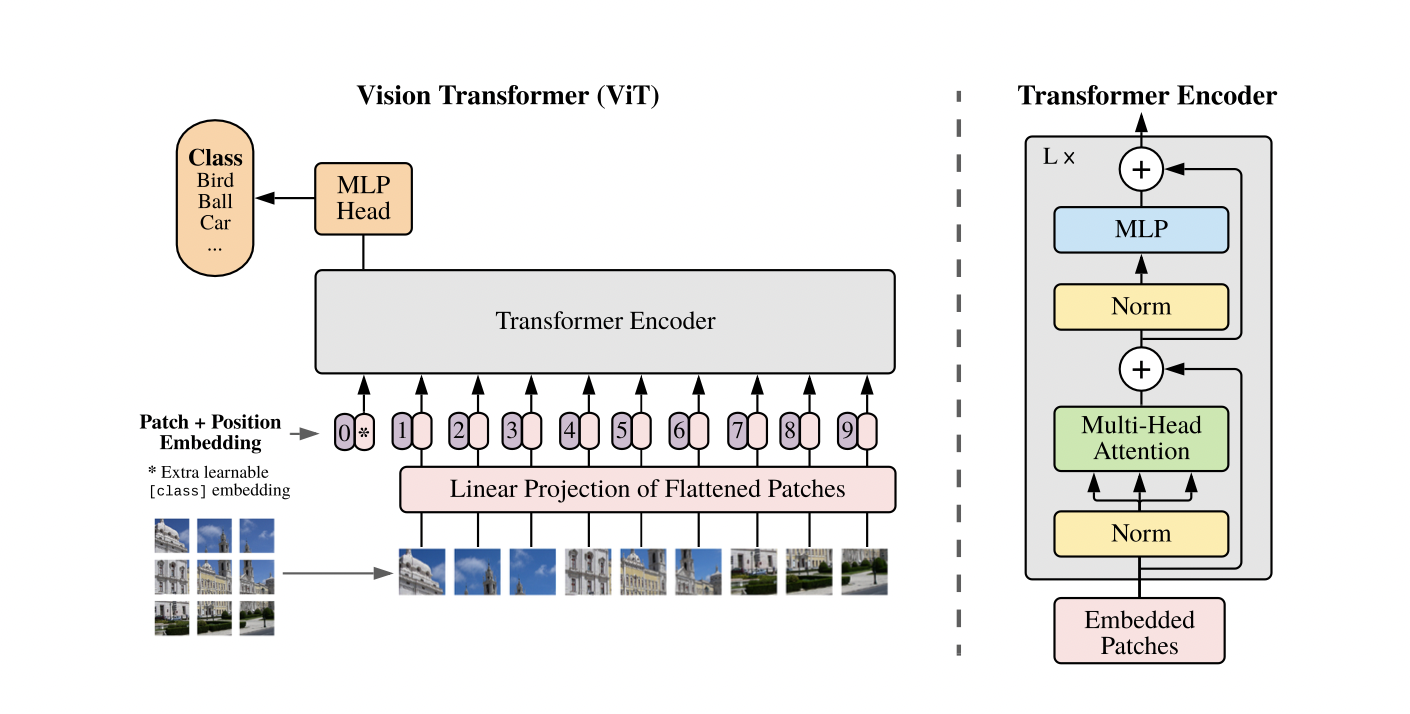
\includegraphics[width=0.8\textwidth]{figure/lmu-vit.png}\\
  \citebutton{Source: Dosovitskiy et al., 2020}{https://arxiv.org/abs/2010.11929}
\end{figure}
\end{frame}

\begin{frame}{ViT Method: Images as Sequences of Patches}
\begin{itemize}
  \item In NLP, the Transformer input is a 1-dimensional sequence of token embeddings; images are 2-dimensional objects.
  \item To stay as close as possible to the original architecture, an image $x \in \mathbb{R}^{H \times W \times C}$ is reshaped into a sequence of flattened 2D patches $x_p \in \mathbb{R}^{N \times (P^2 \cdot C)}$:
  \begin{itemize}
    \item $(H, W)$: resolution of the original image, $C$: number of channels,
    \item $(P, P)$: resolution of each patch (usually $16 \times 16$),
    \item $N = HW/P^2$: number of patches --- the Transformer's effective input sequence length.
  \end{itemize}
  \item The Transformer uses a fixed vector size $D$ through all layers: the flattened patches are mapped to $D$ dimensions with a trainable linear projection $\Rightarrow$ \textbf{patch embeddings}.
\end{itemize}
\end{frame}

\begin{frame}{ViT Method: Class Token and Position Embeddings}
\small% fit16:9
\[
\mathbf{z}_{0} = \left[\mathbf{x}_{\text{class}};\, \mathbf{x}_{p}^{1}\mathbf{E};\, \mathbf{x}_{p}^{2}\mathbf{E};\, \cdots;\, \mathbf{x}_{p}^{N}\mathbf{E}\right] + \mathbf{E}_{pos},
\qquad \mathbf{E} \in \mathbb{R}^{(P^{2} \cdot C) \times D},\; \mathbf{E}_{pos} \in \mathbb{R}^{(N+1) \times D}
\]
\begin{itemize}
  \item A learnable \texttt{[class]} token is prepended to the patch embeddings --- \textbf{like in BERT}.
  \item Its state at the output of the encoder, after layer norm, is the image representation:
  \[ \mathbf{y} = \operatorname{LN}\left(\mathbf{z}_{L}^{0}\right) \]
  \item The classification head is attached only to this token: an MLP with one hidden layer during pre-training, a single linear layer at fine-tuning time.
  \item Standard learnable 1-dimensional \textbf{position embeddings} are added to the patch embeddings.
\end{itemize}
\end{frame}

\begin{frame}{ViT Method: The Encoder}
\begin{itemize}
  \item The standard Transformer encoder: alternating layers of multi-headed self-attention (MSA) and MLP blocks, layer norm (LN) before each block, a residual connection after each block:
\end{itemize}
\[
\mathbf{z}_{\ell}^{\prime} = \operatorname{MSA}\left(\operatorname{LN}\left(\mathbf{z}_{\ell-1}\right)\right) + \mathbf{z}_{\ell-1}, \qquad \ell = 1 \ldots L
\]
\[
\mathbf{z}_{\ell} = \operatorname{MLP}\left(\operatorname{LN}\left(\mathbf{z}_{\ell}^{\prime}\right)\right) + \mathbf{z}_{\ell}^{\prime}, \qquad \ell = 1 \ldots L
\]
% [O] cross-reference to session 9 (original text); EVA-02 and ViT-22B verified 2026-10-18
\vfill
{\footnotesize Newer ViTs update this block as discussed in session 9, e.g.\ SwiGLU and RoPE \citebutton{EVA-02}{https://arxiv.org/abs/2303.11331}, QK-norm and parallel layers \citebutton{ViT-22B}{https://arxiv.org/abs/2302.05442}.\par}
\end{frame}

% Moved here from the HF section below so the term is defined before first use.
% Source: HF CV course, unit3/vision-transformers-for-image-classification
\begin{frame}{CNNs vs.\ Vision Transformers: Inductive Bias}
\small% fit16:9
\begin{itemize}
  \item \textbf{Inductive bias}: the set of assumptions a learning algorithm uses to make predictions --- a shortcut that helps a model make educated guesses based on what it has seen so far.
  \item Two inductive biases of CNNs:
  \begin{itemize}
    \item \textbf{Translational equivariance}: an object can appear anywhere in the image, and CNNs can detect its features.
    \item \textbf{Locality}: pixels interact mainly with their surrounding pixels to form features.
  \end{itemize}
  \item ViT does not have these assumptions. That is why, up to a certain dataset size, CNNs are actually better than ViT.
  \item But: being (mostly) different types of linear functions, the Transformer makes ViT highly scalable --- which lets ViT overcome the missing inductive biases with massive amounts of data.
\end{itemize}
\end{frame}

\begin{frame}{ViT Method: Inductive Bias}
\begin{itemize}
  \item ViT has a significantly lower image-specific inductive bias than CNNs:
  \begin{itemize}
    \item only the MLP layers are local and translationally equivariant; the self-attention layers are global;
    \item the 2-dimensional neighborhood structure is used sparingly: the image is cut into patches at the beginning, and position embeddings are resized as needed at fine-tuning time.
  \end{itemize}
  \item Resolution adjustment and patch extraction are the \emph{only} points where an inductive bias about the 2D structure of images is injected manually.
  \item Alternative (hybrid): the input sequence can be a CNN's feature map, on which the patch embedding projection is applied.
\end{itemize}
\end{frame}

\begin{frame}{ViT: Pre-Training and Fine-Tuning}
\begin{itemize}
  \item Vision Transformers are pre-trained on large datasets and fine-tuned to (smaller) downstream tasks.
  \item For fine-tuning, the pre-training projection head is removed and a zero-initialized $D \times K$ feed-forward layer is attached, $K$ = number of downstream classes.
  \item It is beneficial to fine-tune at a higher resolution than in pre-training; ViT can handle arbitrary sequence lengths.
\end{itemize}
\end{frame}

\begin{frame}{ViT: Experiments}
\begin{itemize}
  \item Similarly to BERT, multiple versions at various scales: Base (B), Large (L), Huge (H) with 12, 24 and 32 layers and 86M, 307M and 632M parameters.
  \item Compared on ImageNet against a slightly modified ResNet, ``ResNet (BiT)'' (group normalization, standardized convolutions), and Noisy Student, a large EfficientNet \citebutton{Xie et al., 2019}{https://arxiv.org/abs/1911.04252}:
  \begin{itemize}
    \item ViT-Huge with $14\times14$ patches: 88.5\,\% accuracy,
    \item ResNet (BiT): 87.54\,\%, Noisy Student: 88.4\,\%,
    \item ViT-Large with $16\times16$ patches: 87.76\,\%.
  \end{itemize}
  \item ViT outperforms CNN-based architectures on all larger datasets, yet performs slightly worse than CNNs on smaller datasets.
\end{itemize}
\end{frame}

%%%%%%%%%%%%%%%%%%%%%%%%%%%%%%%%%%%%%%%%%%%%%%%%%%%%%%%%%%%%%%%%%%
\section{Vision Transformers for Image Classification}
% Source: HF CV course, unit3/vision-transformers/vision-transformers-for-image-classification
%%%%%%%%%%%%%%%%%%%%%%%%%%%%%%%%%%%%%%%%%%%%%%%%%%%%%%%%%%%%%%%%%%

\begin{frame}{Transfer Learning \& Fine-Tuning}
\begin{itemize}
  \item Training a ViT on millions of images is not feasible for everyone. Instead, use openly available pre-trained weights (e.g.\ the Hugging Face Hub).
  \item \textbf{Transfer learning}: leverage the features a ViT learned on a very large dataset and apply them to our (possibly small) dataset.
  \begin{itemize}
    \item By freezing most of the weights, we train only certain layers: good performance with less training time and low GPU consumption.
  \end{itemize}
  \item \textbf{Fine-tuning}: if our domain differs from the pre-training data, update the weights of the entire pre-trained model, with a lower learning rate.
  \item In most scenarios, transfer learning is ample for Vision Transformers.
  \item Both work for \textbf{multi-class} (one label per image) and \textbf{multi-label} (several labels per image) classification.
\end{itemize}
\end{frame}

%%%%%%%%%%%%%%%%%%%%%%%%%%%%%%%%%%%%%%%%%%%%%%%%%%%%%%%%%%%%%%%%%%
\section{Swin Transformer}
% Source: HF CV course, unit3/vision-transformers/swin-transformer
%%%%%%%%%%%%%%%%%%%%%%%%%%%%%%%%%%%%%%%%%%%%%%%%%%%%%%%%%%%%%%%%%%

\begin{frame}{Swin Transformer}
\begin{itemize}
  \item Introduced in 2021 \citebutton{Liu et al., 2021}{https://arxiv.org/abs/2103.14030}: optimizes for latency and performance using a \textbf{shifted window} (as opposed to sliding window) approach, which reduces the number of operations required.
  \item Swin is a \textbf{hierarchical backbone} for computer vision, e.g.\ for image classification.
  \begin{itemize}
    \item A \textit{backbone} is the part of a network that does feature extraction; additional layers can be added on top for a variety of vision tasks.
    \item \textit{Hierarchical} backbones have tiered structures, sometimes with varying resolutions --- in contrast to the non-hierarchical \textit{plain} backbone of e.g.\ ViTDet.
  \end{itemize}
\end{itemize}
\end{frame}

\begin{frame}{Shifted Windows}
\begin{itemize}
  \item In the original ViT, attention is done between each patch and all other patches --- computationally intensive.
  \item Swin reduces ViT's quadratic complexity to \textbf{linear} complexity (w.r.t.\ image size): similar to a CNN, patches only attend to other patches in the \textbf{same window}, and are then gradually merged with neighboring patches. This is what makes Swin hierarchical.
\end{itemize}
\begin{figure}
  \centering
  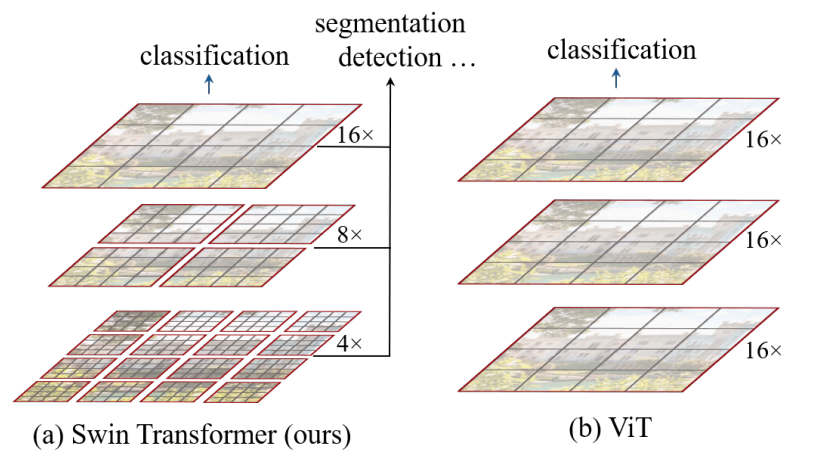
\includegraphics[width=0.42\textwidth]{figure/swin-vs-vit.png}\\
  \citebutton{Source: Liu et al., 2021}{https://arxiv.org/abs/2103.14030}
\end{figure}
\end{frame}

\begin{frame}{Swin: Advantages and Successors}
\begin{itemize}
  \item \textbf{Computational efficiency}: Swin is more performant than completely patch-based approaches like ViT.
  \item \textbf{Large datasets}: as training size goes up, Swin outperforms CNNs; the large number of parameters enables increased capacity for learning more complex representations.
  \item \textbf{Swin Transformer V2} \citebutton{Liu et al., 2022}{https://arxiv.org/abs/2111.09883}: one of the first 3B-parameter vision models, trainable with high-resolution images. It stabilizes training, transfers models pre-trained on low-resolution images to high-resolution tasks, and uses SimMIM, a self-supervised approach that reduces the number of labeled images required.
  \item \textbf{Image restoration}: SwinIR turns low-resolution into high-resolution images; Swin2SR improves on it using Swin V2.
\end{itemize}
\end{frame}

%%%%%%%%%%%%%%%%%%%%%%%%%%%%%%%%%%%%%%%%%%%%%%%%%%%%%%%%%%%%%%%%%%
\section{DEtection TRansformer (DETR)}
% Source: HF CV course, unit3/vision-transformers/detr
%%%%%%%%%%%%%%%%%%%%%%%%%%%%%%%%%%%%%%%%%%%%%%%%%%%%%%%%%%%%%%%%%%

\begin{frame}{Object Detection with DETR}
\begin{itemize}
  \item \textbf{Object detection}: detect objects in an image. Input: e.g.\ an image of a road. Output: e.g.\ \texttt{[('car',X1,Y1,W1,H1), ('pedestrian',X2,Y2,W2,H2)]} --- class, plus the $x,y$ coordinates, width and height of each bounding box.
  \item Traditional detectors like YOLO use hand-crafted features such as \textbf{anchor box priors} (initial guesses of object locations and shapes), and post-processing steps to remove overlapping boxes, which need carefully selected filtering heuristics.
  \item \textbf{DETR} \citebutton{Carion et al., 2020}{https://arxiv.org/abs/2005.12872} simplifies the detector: an encoder-decoder Transformer after the feature-extraction backbone \textbf{directly predicts bounding boxes in parallel}, requiring minimal post-processing.
\end{itemize}
\end{frame}

\begin{frame}{DETR: Architecture}
\begin{figure}
  \centering
  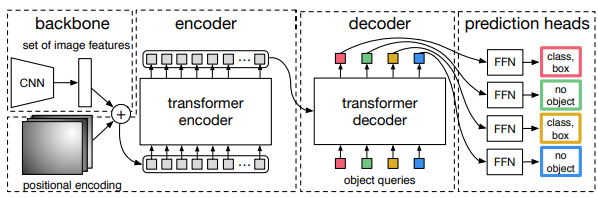
\includegraphics[width=0.61\textwidth]{figure/detr-architecture.png}\\
  \citebutton{Source: Carion et al., 2020}{https://arxiv.org/abs/2005.12872}
\end{figure}
\begin{itemize}
  \item A CNN backbone; its output is fed into a Transformer encoder, resulting in $N$ embeddings.
  \item The decoder uses learned positional embeddings (\textbf{object queries}) and the encoder output, generating another $N$ embeddings.
  \item Each of the $N$ embeddings goes through feed-forward layers predicting the bounding box (coordinates, width, height) and the object class --- or that there is no object.
\end{itemize}
\end{frame}

\begin{frame}{DETR: Encoder-Decoder}
\begin{itemize}
  \item The encoder expects a sequence, so the backbone's feature map of size \texttt{[dimension, height, width]} is downsized and flattened to \texttt{[dimension, less than height $\times$ width]}.
\end{itemize}
\begin{figure}
  \centering
  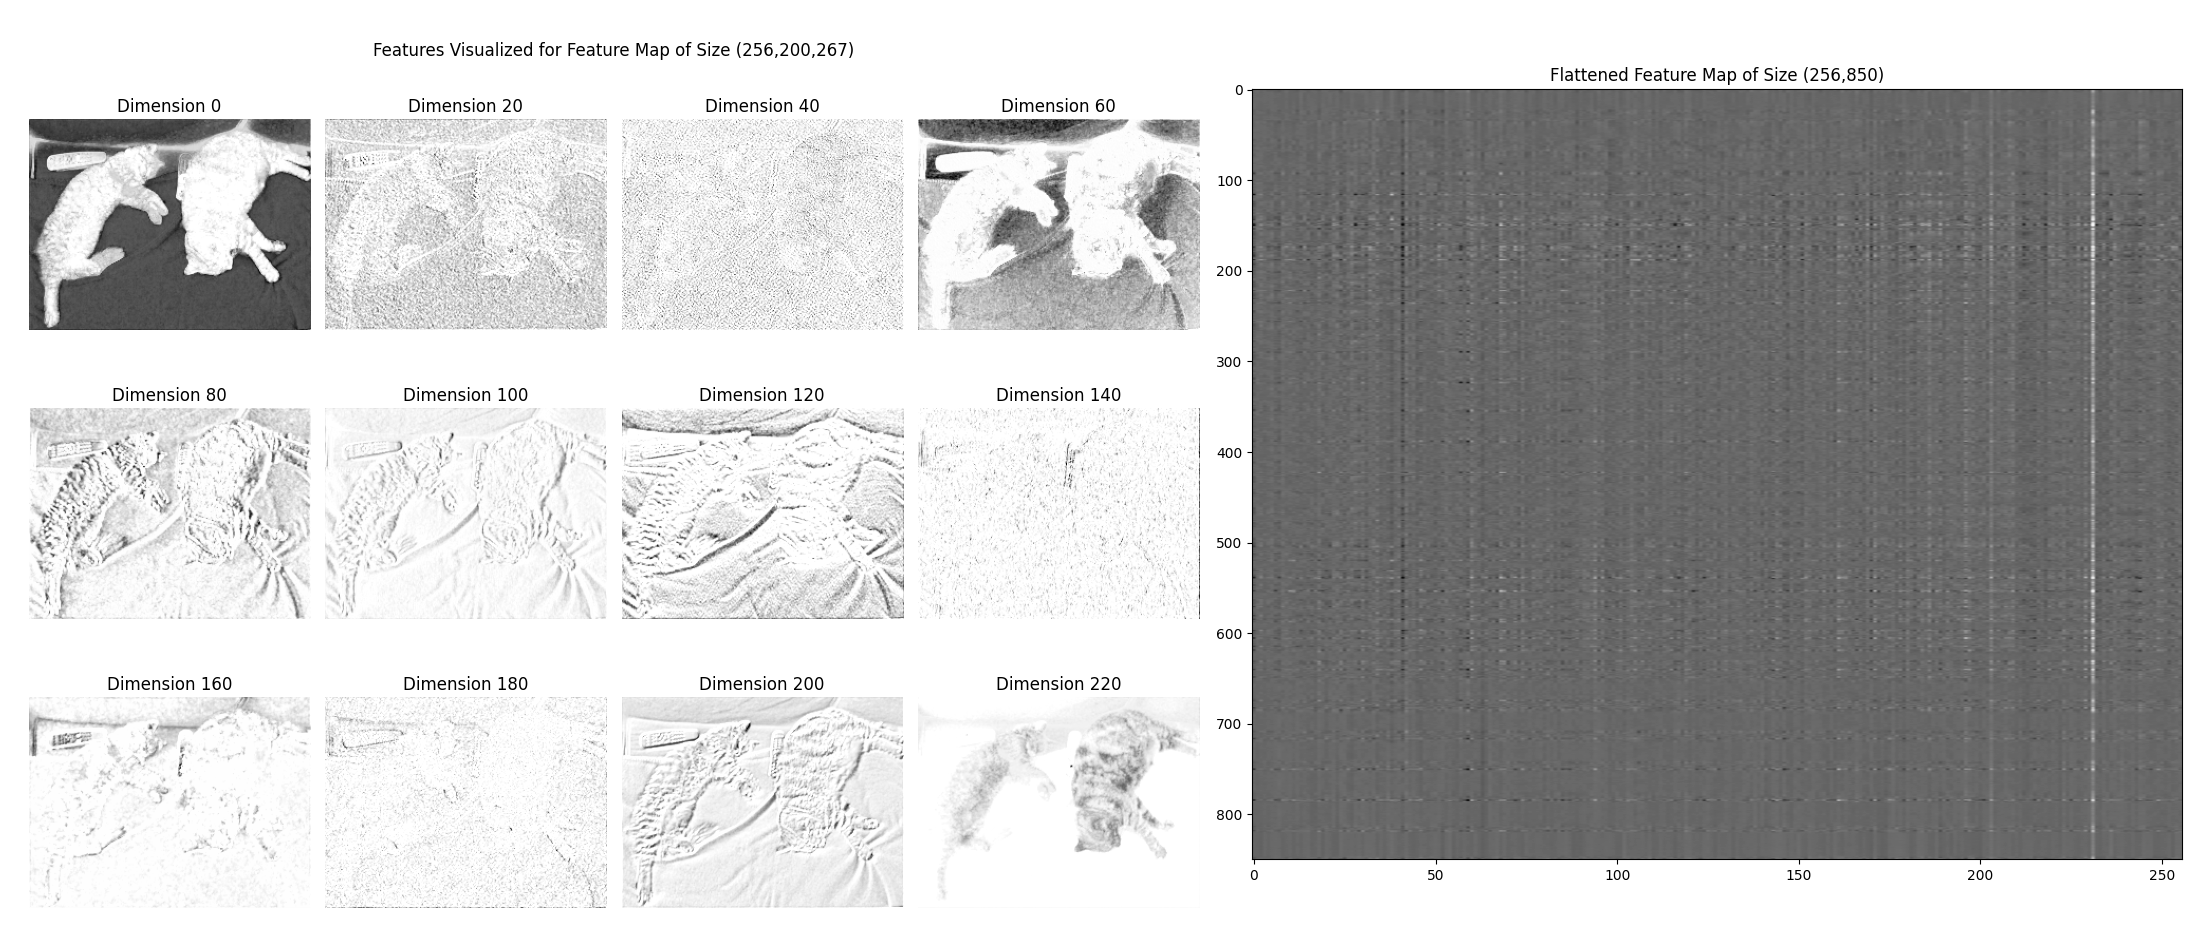
\includegraphics[width=0.7\textwidth]{figure/detr-feature-maps.png}
\end{figure}
{\footnotesize Left: 12 of 256 feature-map dimensions; each extracts some features of the cat image (some focus on the cat's patterns, some on the bed sheets). Right: keeping 256 dimensions, width and height are flattened into size 850.}
\end{frame}

\begin{frame}{DETR: Positional Embeddings}
\begin{itemize}
  \item Transformers are permutation invariant, so positional embeddings are added in both encoder and decoder to remind the model where in the image an embedding comes from.
  \item \textbf{Encoder: fixed} positional encodings, as in the original Transformer --- sinusoidal functions of varying frequencies at different feature dimensions. A sense of position without learned parameters.
  \item \textbf{Decoder: learned} positional encodings (the object queries) --- each position has its own encoding, learned during training.
\end{itemize}
\end{frame}

\begin{frame}{DETR: Set-Based Global Loss}
\footnotesize% fit16:9

\begin{itemize}
  \item YOLO's loss: bounding box, objectness (probability that an object exists in a region of interest) and class loss, computed over a fixed number of boxes per grid cell.
  \item DETR generates unique bounding boxes in a \textbf{permutation-invariant} manner: the order of the detections does not matter, and the boxes must differ from each other. So predictions must be \textbf{matched} to the ground truth before they can be scored.
  \item \textbf{Bipartite matching}: a one-to-one matching between ground-truth and predicted boxes, pairing those with the highest similarity in box and class.
  \begin{itemize}
    \item The closest prediction is matched with the corresponding ground truth, so boxes and classes are adjusted properly in the loss.
    \item Without matching, a correct prediction that is not in the same order as the ground truth would be marked incorrect.
  \end{itemize}
\end{itemize}
\end{frame}

%%%%%%%%%%%%%%%%%%%%%%%%%%%%%%%%%%%%%%%%%%%%%%%%%%%%%%%%%%%%%%%%%%
\section{Transformer-Based Image Segmentation}
% Source: HF CV course, unit3/vision-transformers/vision-transformers-for-image-segmentation
%%%%%%%%%%%%%%%%%%%%%%%%%%%%%%%%%%%%%%%%%%%%%%%%%%%%%%%%%%%%%%%%%%

\begin{frame}{CNNs vs.\ Transformers for Segmentation}
\small% fit16:9
Before ViTs, CNNs (U-Net, Mask R-CNN) were the go-to choice for segmentation. Limitations Transformers aim to solve:
\begin{itemize}
  \item \textbf{Spatial limitations}: CNNs learn local patterns through small receptive fields, so it is hard to link features that are far apart but related. ViTs capture global dependencies via attention, considering the entire image at once.
  \item \textbf{Task-specific components}: Mask R-CNN uses hand-designed components (e.g.\ spatial anchors) that add complexity and require manual tuning. ViT-based methods eliminate them.
  \item \textbf{Task specialization}: CNN-based models treat semantic, instance and panoptic segmentation separately. ViT-based models such as MaskFormer, SegFormer or SAM handle all three in a single framework.
\end{itemize}
\end{frame}

\begin{frame}{MaskFormer}
\begin{figure}
  \centering
  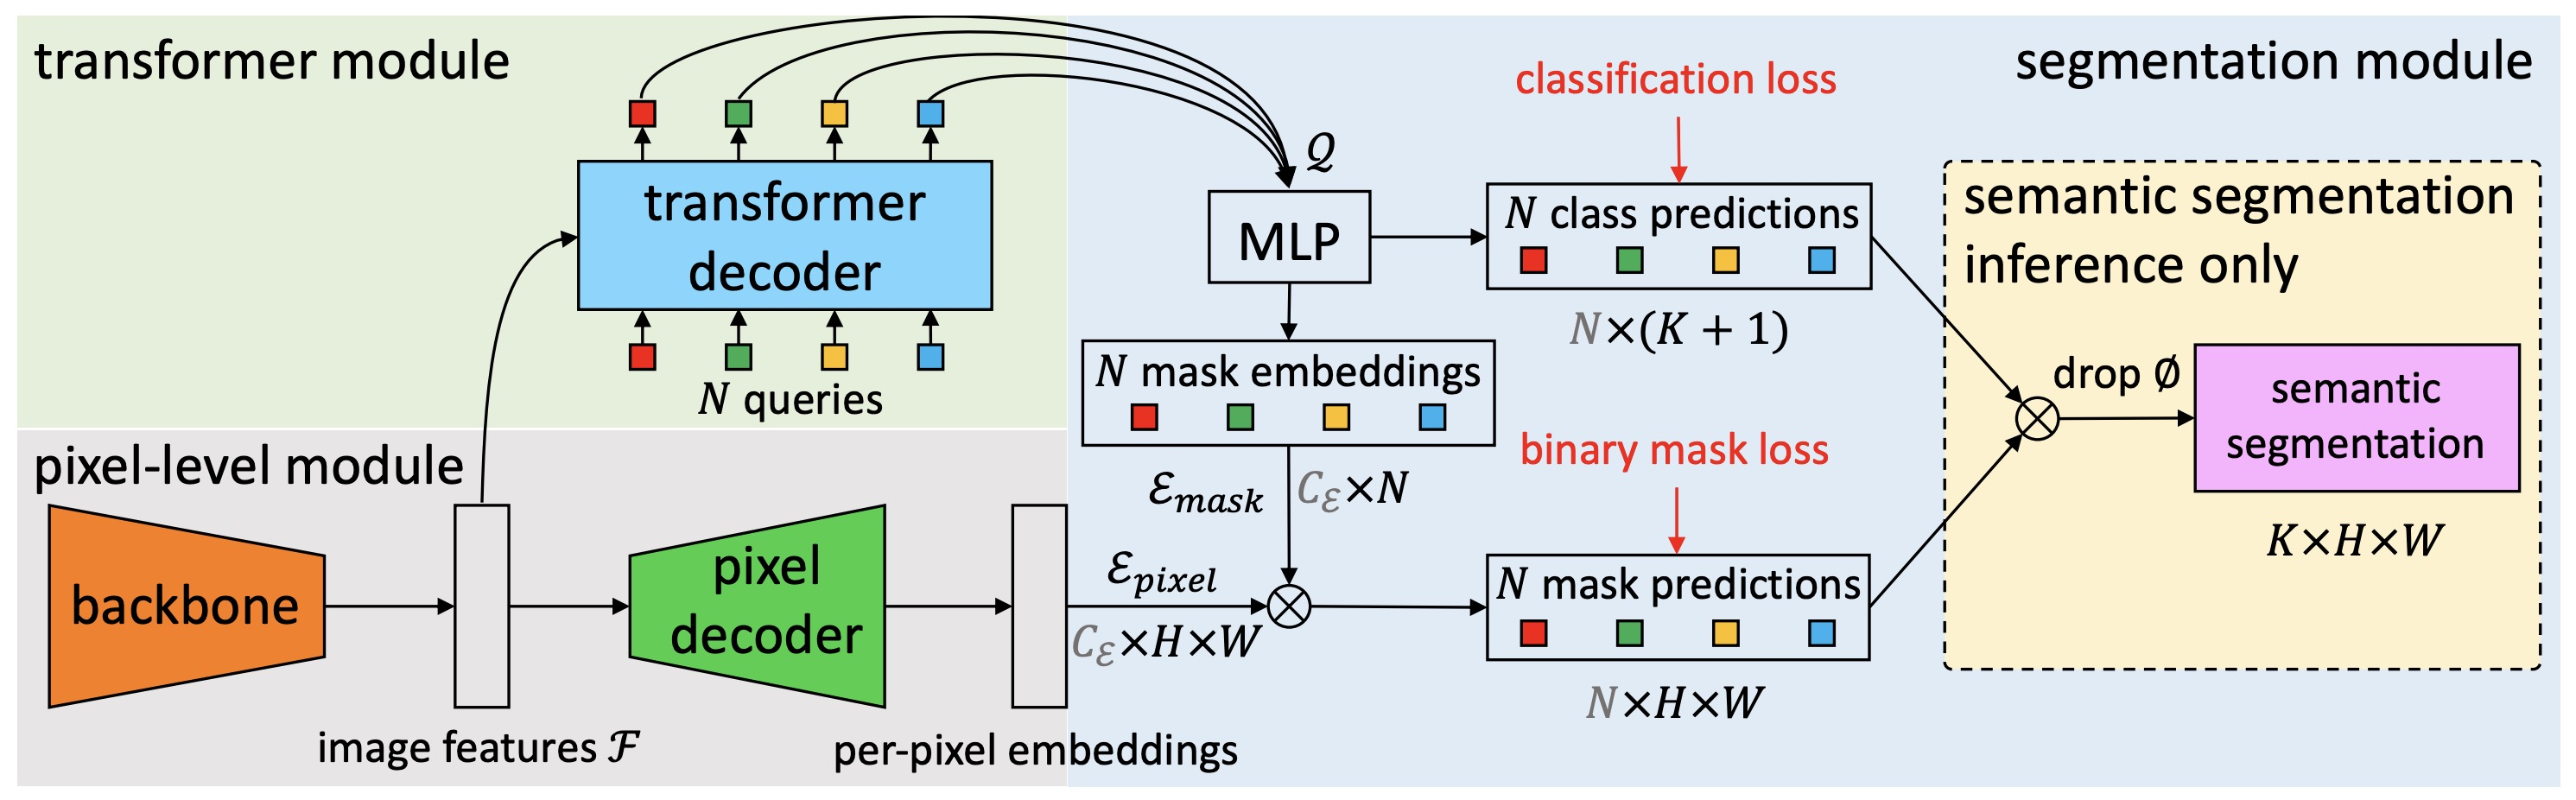
\includegraphics[width=0.62\textwidth]{figure/maskformer-architecture.jpg}\\
  \citebutton{Source: Cheng et al., 2021}{https://arxiv.org/abs/2107.06278}
\end{figure}
\vspace{-0.2cm}
{\small
\begin{itemize}
  \item \textbf{Pixel-level module}: a backbone extracts image features; a pixel decoder generates per-pixel embeddings.
  \item \textbf{Transformer module}: a standard Transformer decoder computes per-segment embeddings from image features and learnable queries.
  \item \textbf{Segmentation module}: class predictions (linear classifier) and mask embeddings (MLP) per segment; mask embeddings combined with per-pixel embeddings give a binary mask per segment.
\end{itemize}
}
\end{frame}

\begin{frame}{MaskFormer: Training and Fine-Tuning}
\small% fit16:9
\begin{itemize}
  \item MaskFormer predicts segmentation masks for each class present in an image, unifying semantic and instance segmentation in one architecture.
  \item Trained with a binary mask loss --- the same one as DETR --- plus a cross-entropy classification loss per predicted segment.
  \item \textbf{Panoptic segmentation}: label every pixel with its category \textit{and} identify distinct objects within those categories (semantic + instance). MaskFormer's output contains multiple instances of the same class, each with its own mask.
  \item Transformer-based segmentation models are data-hungry and hard to train from scratch, so transfer learning is common: typically the backbone, the pixel decoder and the Transformer decoder are frozen, and the rest is fine-tuned for new class predictions and masks.
\end{itemize}
\end{frame}

%%%%%%%%%%%%%%%%%%%%%%%%%%%%%%%%%%%%%%%%%%%%%%%%%%%%%%%%%%%%%%%%%%
\section{Exploring Multimodal Text and Vision Models}
% Source: HF CV course, unit4/multimodal-models/pre-intro (course-navigation parts not used)
%%%%%%%%%%%%%%%%%%%%%%%%%%%%%%%%%%%%%%%%%%%%%%%%%%%%%%%%%%%%%%%%%%

\begin{frame}{From Vision to Multimodality}
\begin{itemize}
  \item The Transformer architecture revolutionized NLP, but did not stop at the text modality.
  \item It has begun to conquer the field of vision (including image and video), bringing with it a wide array of new research and applications.
  \item Next: the \textbf{data fusion} possibilities that the modality-overlapping use of Transformers has enabled, and the tasks and models that benefit:
  \begin{itemize}
    \item why blending text and images is crucial;
    \item multimodal tasks such as image-to-text, text-to-image, visual question answering (VQA), captioning, visual reasoning;
    \item vision language models such as CLIP and its relatives.
  \end{itemize}
\end{itemize}
\end{frame}

%%%%%%%%%%%%%%%%%%%%%%%%%%%%%%%%%%%%%%%%%%%%%%%%%%%%%%%%%%%%%%%%%%
\section{A Multimodal World}
% Source: HF CV course, unit4/multimodal-models/a_multimodal_world
% (the Mehrabian 7-38-55 paragraph and the search-engine history are not used)
%%%%%%%%%%%%%%%%%%%%%%%%%%%%%%%%%%%%%%%%%%%%%%%%%%%%%%%%%%%%%%%%%%

\begin{frame}{What Is Multimodality?}
\begin{itemize}
  \item A \textbf{modality} is a medium or a way in which something exists or is done.
  \item Humans use 5 sense organs; each is a different modality through which information comes to us --- hence \emph{multimodality}.
  \item Example: on a windy night you hear an eerie sound. Relying on your ears alone, you cannot tell its source; once you turn on the lights and look around, you see a half-open window.
  \item Adding modalities to the same situation lets them assist each other and improves the information content.
\end{itemize}
\end{frame}

\begin{frame}{Modalities in Deep Learning}
\begin{itemize}
  \item In deep learning, each modality is a way data arrives to a model. Most common: \textbf{vision, audio, text}; others for specific use cases: LIDAR, EEG data, eye-tracking data, \ldots
  \item Unimodal models and datasets have been studied for long, with many tasks and benchmarks, but are limited: a single modality might not give the complete picture.
  \item Combining modalities increases the information content and reduces the chance of missing cues.
  \item Common combinations:
  \begin{itemize}
    \item vision + text: infographics, memes, articles, blogs;
    \item vision + audio: a video call, dyadic conversations;
    \item vision + audio + text: videos or movies with captions, social media content;
    \item audio + text: voice notes, music files with lyrics.
  \end{itemize}
\end{itemize}
\end{frame}

\begin{frame}{Multimodal Datasets and Tasks}
\small% fit16:9
\begin{itemize}
  \item A dataset with multiple modalities is a \textbf{multimodal dataset}, e.g.
  \begin{itemize}
    \item vision + text: Visual Storytelling, Visual Question Answering, LAION-5B;
    \item vision + audio: VGG-Sound, RAVDESS; vision + audio + text: RECOLA, IEMOCAP.
  \end{itemize}
  \item A task involving two or more modalities is a \textbf{multimodal task}; typically, two different modalities at the input and output ends:
  \begin{itemize}
    \item vision + text: visual question answering, image-to-text (captioning, OCR), text-to-image (generation), text-to-video;
    \item audio + text: automatic speech recognition, text-to-speech.
  \end{itemize}
  \item Example: multimodal emotion recognition from audio+text, text+vision, audio+vision or all three is more efficient than unimodal emotion recognition.
\end{itemize}
\end{frame}

\begin{frame}{Multimodal Models: Fusion}
\begin{figure}
  \centering
  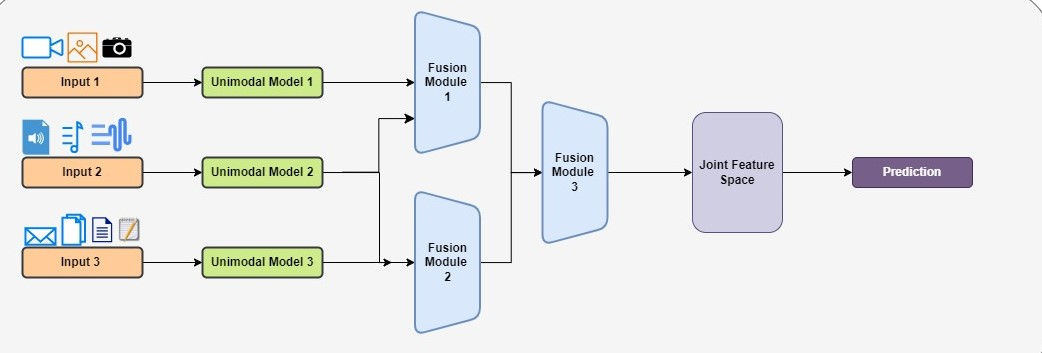
\includegraphics[width=0.85\textwidth]{figure/hf-multimodal-model.jpg}
\end{figure}
\small
\begin{itemize}
  \item A \textbf{multimodal model} processes data from multiple modalities at the same time.
  \item Unimodal models encode each input; a \textbf{fusion module} combines the encoded data (early, late, or hybrid fusion) into a joint representation; a classification network makes predictions from it.
\end{itemize}
\end{frame}

\begin{frame}{Application: Multimodal Search}
\begin{itemize}
  \item Online content is largely multimodal: an image comes with text that describes it; many companies hold large, multimodal, mostly unstructured databases.
  \item \textbf{Vision language models (VLMs)} understand and process both vision and text and can serve as candidates for multimodal search.
  \item Idea: map text and image pairs to a \textbf{joint embedding space} where image and text embeddings that are similar in meaning lie close together.
  \item This enables text-to-image search and vice versa, and other downstream tasks on the same embeddings.
\end{itemize}
\end{frame}

%%%%%%%%%%%%%%%%%%%%%%%%%%%%%%%%%%%%%%%%%%%%%%%%%%%%%%%%%%%%%%%%%%
\section{Multimodal Architectures}
% Source: LMU Multimodal Deep Learning booklet, ch. 3 overview (02-00-multimodal.Rmd). CC BY-NC-SA 4.0.
%%%%%%%%%%%%%%%%%%%%%%%%%%%%%%%%%%%%%%%%%%%%%%%%%%%%%%%%%%%%%%%%%%

\begin{frame}{Multimodal Architectures: Overview}
\begin{itemize}
  \item \textbf{Multimodal learning}: learning representations from different types of input modalities, such as image data, text or speech.
  \item Methodological breakthroughs in NLP and computer vision made multimodal models attractive: they strengthen predictions and better emulate the way humans learn.
  \item With images and text as input data, five families:
  \begin{enumerate}
    \item \textbf{Image2Text}: e.g.\ captioning
    \item \textbf{Text2Image}: generating images from text
    \item \textbf{Images supporting language models}
    \item \textbf{Text supporting vision models}
    \item \textbf{Models for both modalities}
  \end{enumerate}
\end{itemize}
\end{frame}

\begin{frame}{Image2Text}
\begin{itemize}
  \item \textbf{Image2Text}: describing a photograph or parsing a complex scene is easy for humans, much harder for computers.
  \begin{itemize}
    \item MS COCO (\emph{Common Objects in Context}, 2014) addresses three core problems in scene understanding: object detection, segmentation, and captioning.
    \item Transformer-based architectures, e.g.\ the Meshed-Memory Transformer ($M^2$), improve both image encoding and language generation for captioning.
  \end{itemize}
\end{itemize}
\end{frame}

\begin{frame}{Text2Image}
\begin{itemize}
  \item \textbf{Text2Image}: incorporating textual input to generate visual representations.
  \begin{itemize}
    \item Made possible largely by NLP breakthroughs in contextual text representations: Transformer-like architectures encode the input into embedding vectors that guide image generation.
    \item Roots: GANs, VAEs, VQ-VAE, diffusion, and autoregressive models.
  \end{itemize}
\end{itemize}
\end{frame}

\begin{frame}{Images Supporting Language Models}
\begin{itemize}
  \item Distributional models such as word2vec and BERT assume that meaning comes from the context in which words appear in a text corpus.
  \item Historically questioned: words and sentences must be \textbf{grounded} in other perceptual dimensions to understand their meaning.
  \item Starting point: a language model into which visual representations are integrated. A spectrum of solutions:
  \begin{itemize}
    \item textual and visual elements learned separately, then combined;
    \item textual and visual features learned jointly.
  \end{itemize}
  \item Often better than pure language models, but they still struggle, e.g.\ with abstract words and sentences.
\end{itemize}
\end{frame}

\begin{frame}{Text Supporting Vision Models}
\begin{itemize}
  \item Natural language as additional supervision for computer vision models: much more signal than in manually labeled data alone.
  \item Prominent example: \textbf{CLIP} (\emph{Contrastive Language-Image Pre-training}), with the WIT dataset of 400 million text-image pairs scraped from the internet.
  \begin{itemize}
    \item A text encoder and an image encoder are pre-trained jointly with a contrastive goal: predict which text belongs to which image in a batch --- more efficient than generating captions.
    \item At test time, the learned text encoder works as a ``zero-shot'' classifier on embeddings of the target dataset's classes.
  \end{itemize}
  \item Inspired by NLP's pre-training directly on raw text (e.g.\ GPT-n).
\end{itemize}
\end{frame}

\begin{frame}{Models for Both Modalities}
\begin{itemize}
  \item Goal: incorporate text and image inputs into a single unifying framework, closer to general self-supervised learning.
  \item Advantages: no human labelling, so no capacity constraints of supervised models; rather than potentially learning modality-specific biases, a general multipurpose framework can help increase robustness while simplifying the learner portfolio.
\end{itemize}
\end{frame}

\begin{frame}{Models for Both Modalities: Examples}
\begin{itemize}
  \item Examples:
  \begin{itemize}
    \item \textbf{data2vec}: one self-supervised framework for speech, language, or vision --- predict latent representations of the full input from a masked view, with a standard Transformer;
    \item \textbf{ViLBERT}: an earlier model that handles cross-modality tasks;
    \item \textbf{Flamingo}: a few-shot model with 80B parameters, using a large language model for open-ended text generation.
  \end{itemize}
\end{itemize}
\end{frame}

%%%%%%%%%%%%%%%%%%%%%%%%%%%%%%%%%%%%%%%%%%%%%%%%%%%%%%%%%%%%%%%%%%
\section{Introduction to Vision Language Models}
% Source: HF CV course, unit4/multimodal-models/vlm-intro
%%%%%%%%%%%%%%%%%%%%%%%%%%%%%%%%%%%%%%%%%%%%%%%%%%%%%%%%%%%%%%%%%%

\begin{frame}{Our World Is Multimodal}
\begin{itemize}
  \item Humans explore the world through diverse senses: sight, sound, touch, scent. Machine learning seeks models that process and integrate data across multiple \textbf{modalities}.
  \item Two key challenges:
  \begin{itemize}
    \item \textbf{Representation}: effectively summarizing multimodal data, capturing the connections among individual modality elements.
    \item \textbf{Alignment}: identifying connections and interactions across all elements.
  \end{itemize}
  \item Inherent difficulties: one modality may dominate the others; additional modalities can introduce noise; full coverage over all modalities is not guaranteed; modalities can have complicated relationships.
  \item This chapter: the fusion of vision and language --- \textbf{Vision Language Models (VLMs)}.
\end{itemize}
\end{frame}

\begin{frame}{From Training from Scratch to Pre-Training}
\small% fit16:9
\begin{itemize}
  \item Generating text from images (captioning, visual question answering) has been studied for years.
  \item A shift from training from scratch to the paradigm first proposed in ULMFiT \citebutton{Howard and Ruder, 2018}{https://aclanthology.org/P18-1031.pdf}:
  \begin{itemize}
    \item pre-train the model with extensive training data,
    \item fine-tune it with task-specific data,
    \item use it for downstream tasks such as classification.
  \end{itemize}
  \item VLMs extend this paradigm to images. In 2021, OpenAI's \textbf{CLIP} used an image-text \textbf{contrastive} objective: paired images and texts are brought close in the embedding space, all others pushed apart.
  \item This captures rich vision-language correspondence, enabling \textbf{zero-shot} predictions by matching embeddings of any image and text. CLIP outperformed ImageNet models on out-of-distribution tasks.
\end{itemize}
\end{frame}

\begin{frame}{VLM Mechanism}
\begin{itemize}
  \item Given image-text pairs: extract features with a text encoder and an image encoder (CNN- or Transformer-based), then learn the vision-language correlation with a pre-training objective:
  \begin{itemize}
    \item \textbf{contrastive}: pull paired samples close, push others far away in the embedding space;
    \item \textbf{generative}: learn semantic features by generating image/text data;
    \item \textbf{alignment}: global image-text matching or local region-word matching.
  \end{itemize}
  \item With the learned correlation, VLMs are evaluated zero-shot by matching embeddings of any given images and texts.
\end{itemize}
\begin{figure}
  \centering
  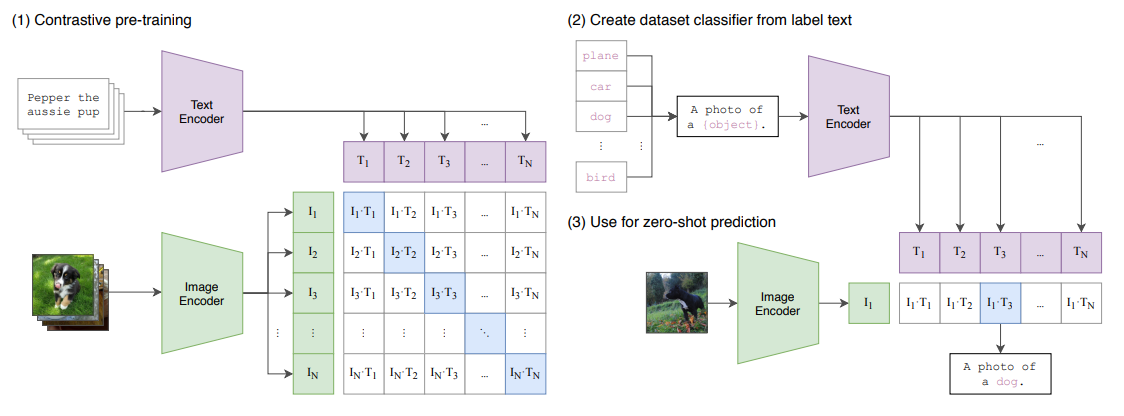
\includegraphics[width=0.27\textwidth]{figure/vlm-clip-mechanism.png}\\
  \citebutton{Source: Radford et al., 2021}{https://arxiv.org/abs/2103.00020}
\end{figure}
\end{frame}

\begin{frame}{VLM Strategies}
\small% fit16:9
Grouping VLMs by how they combine the two modes of learning:
\begin{itemize}
  \item \textbf{Images as tokens}: divide images into patches, treat each patch as a \enquote{token}, and train on joint sequences of text and image tokens (VisualBERT, SimVLM).
  \item \textbf{Image embeddings as a prefix} for a \textit{frozen} pre-trained language model: learn an image embedding space compatible with the language model's, without changing its parameters (Frozen, ClipCap).
  \item \textbf{Cross-attention}: a specially designed cross-attention mechanism fuses visual information into the layers of the language model (VisualGPT).
  \item \textbf{No training}: combine vision and language models via guided decoding of the next token (MAGiC).
\end{itemize}
\vspace{0.2cm}
Research focus: collecting large-scale informative image-text data, designing effective models for big data, and new pre-training objectives.
\end{frame}

\begin{frame}{Common VLM Datasets}
\begin{itemize}
  \item \textbf{MSCOCO}: 328K images, each paired with 5 independent captions.
  \item \textbf{NoCaps}: measures generalization to unseen classes and concepts (in-domain, near-domain, out-of-domain).
  \item \textbf{Conceptual Captions}: 3 million image-caption pairs, mined from the web and post-processed.
  \item \textbf{ALIGN}: a noisy dataset of over one billion image alt-text pairs, without expensive filtering or post-processing.
  \item \textbf{LAION}: image-text pairs extracted from Common Crawl (web pages crawled 2014--2021); used to train Stable Diffusion.
\end{itemize}
\end{frame}

\begin{frame}{Downstream Tasks and Evaluation}
\begin{itemize}
  \item Downstream tasks: image classification, object detection, semantic segmentation, image-text retrieval, action recognition.
  \item \textbf{Zero-shot prediction} (most common): apply the pre-trained VLM directly, without task-specific fine-tuning.
  \item \textbf{Linear probing}: freeze the VLM and train a linear classifier on its embeddings, measuring the quality of the representation.
  \item Harder datasets probe generalization: \textbf{Hateful Memes} adds difficult \enquote{benign confounders}; \textbf{Winoground} tests whether models truly grasp compositional relationships.
\end{itemize}
\begin{figure}
  \centering
  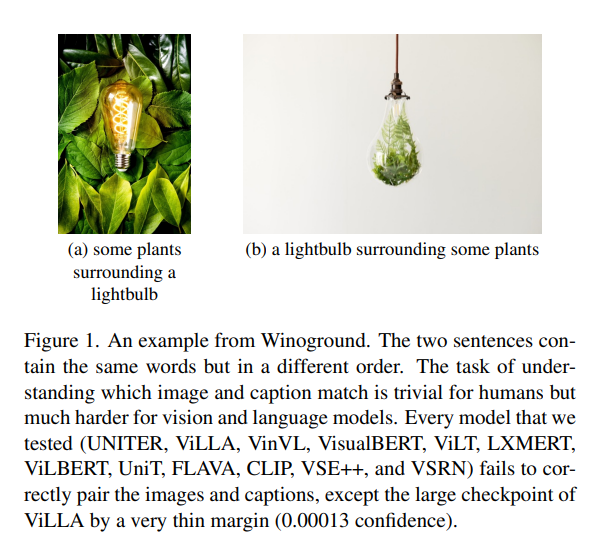
\includegraphics[width=0.20\textwidth]{figure/winoground.png}\\
  \citebutton{Source: Thrush et al., 2022}{https://arxiv.org/abs/2204.03162}
\end{figure}
\end{frame}

%%%%%%%%%%%%%%%%%%%%%%%%%%%%%%%%%%%%%%%%%%%%%%%%%%%%%%%%%%%%%%%%%%
\section{CLIP and Relatives}
% Source: HF CV course, unit4/multimodal-models/clip-and-relatives/Introduction
%%%%%%%%%%%%%%%%%%%%%%%%%%%%%%%%%%%%%%%%%%%%%%%%%%%%%%%%%%%%%%%%%%

\begin{frame}{Before and After CLIP}
\footnotesize% fit16:9

\textbf{Pre-CLIP:}
\begin{itemize}
  \item \textit{Multimodal Deep Learning} (Ngiam et al., 2011): deep learning for multimodal inputs.
  \item \textit{Deep Visual-Semantic Alignments} (Karpathy \& Fei-Fei, 2015): aligning text with specific image regions.
  \item \textit{Show and Tell} (Vinyals et al., 2015): CNNs and RNNs combined to turn images into descriptive language.
\end{itemize}
\textbf{Post-CLIP:}
\begin{itemize}
  \item \textbf{CLIP}: learns from a vast array of internet image-text pairs; zero-shot learning.
  \item \textbf{GroupViT}: segmentation and semantic understanding combined with language.
  \item \textbf{BLIP}: bidirectional learning between vision and language; generating text from images.
  \item \textbf{OWL-ViT}: object-centric representations, understanding objects in images in context with text.
\end{itemize}
\end{frame}

%%%%%%%%%%%%%%%%%%%%%%%%%%%%%%%%%%%%%%%%%%%%%%%%%%%%%%%%%%%%%%%%%%
\section{Losses}
% Source: HF CV course, unit4/multimodal-models/clip-and-relatives/losses
%%%%%%%%%%%%%%%%%%%%%%%%%%%%%%%%%%%%%%%%%%%%%%%%%%%%%%%%%%%%%%%%%%

\begin{frame}{Contrastive Learning}
\begin{itemize}
  \item \textbf{Contrastive learning}: an unsupervised method for representation learning.
  \item Objective: a representation in which similar items are positioned close together and dissimilar items are clearly separated.
  \item Example: keep the representations of dogs close to other dogs, but far from cats.
\end{itemize}
\begin{figure}
  \centering
  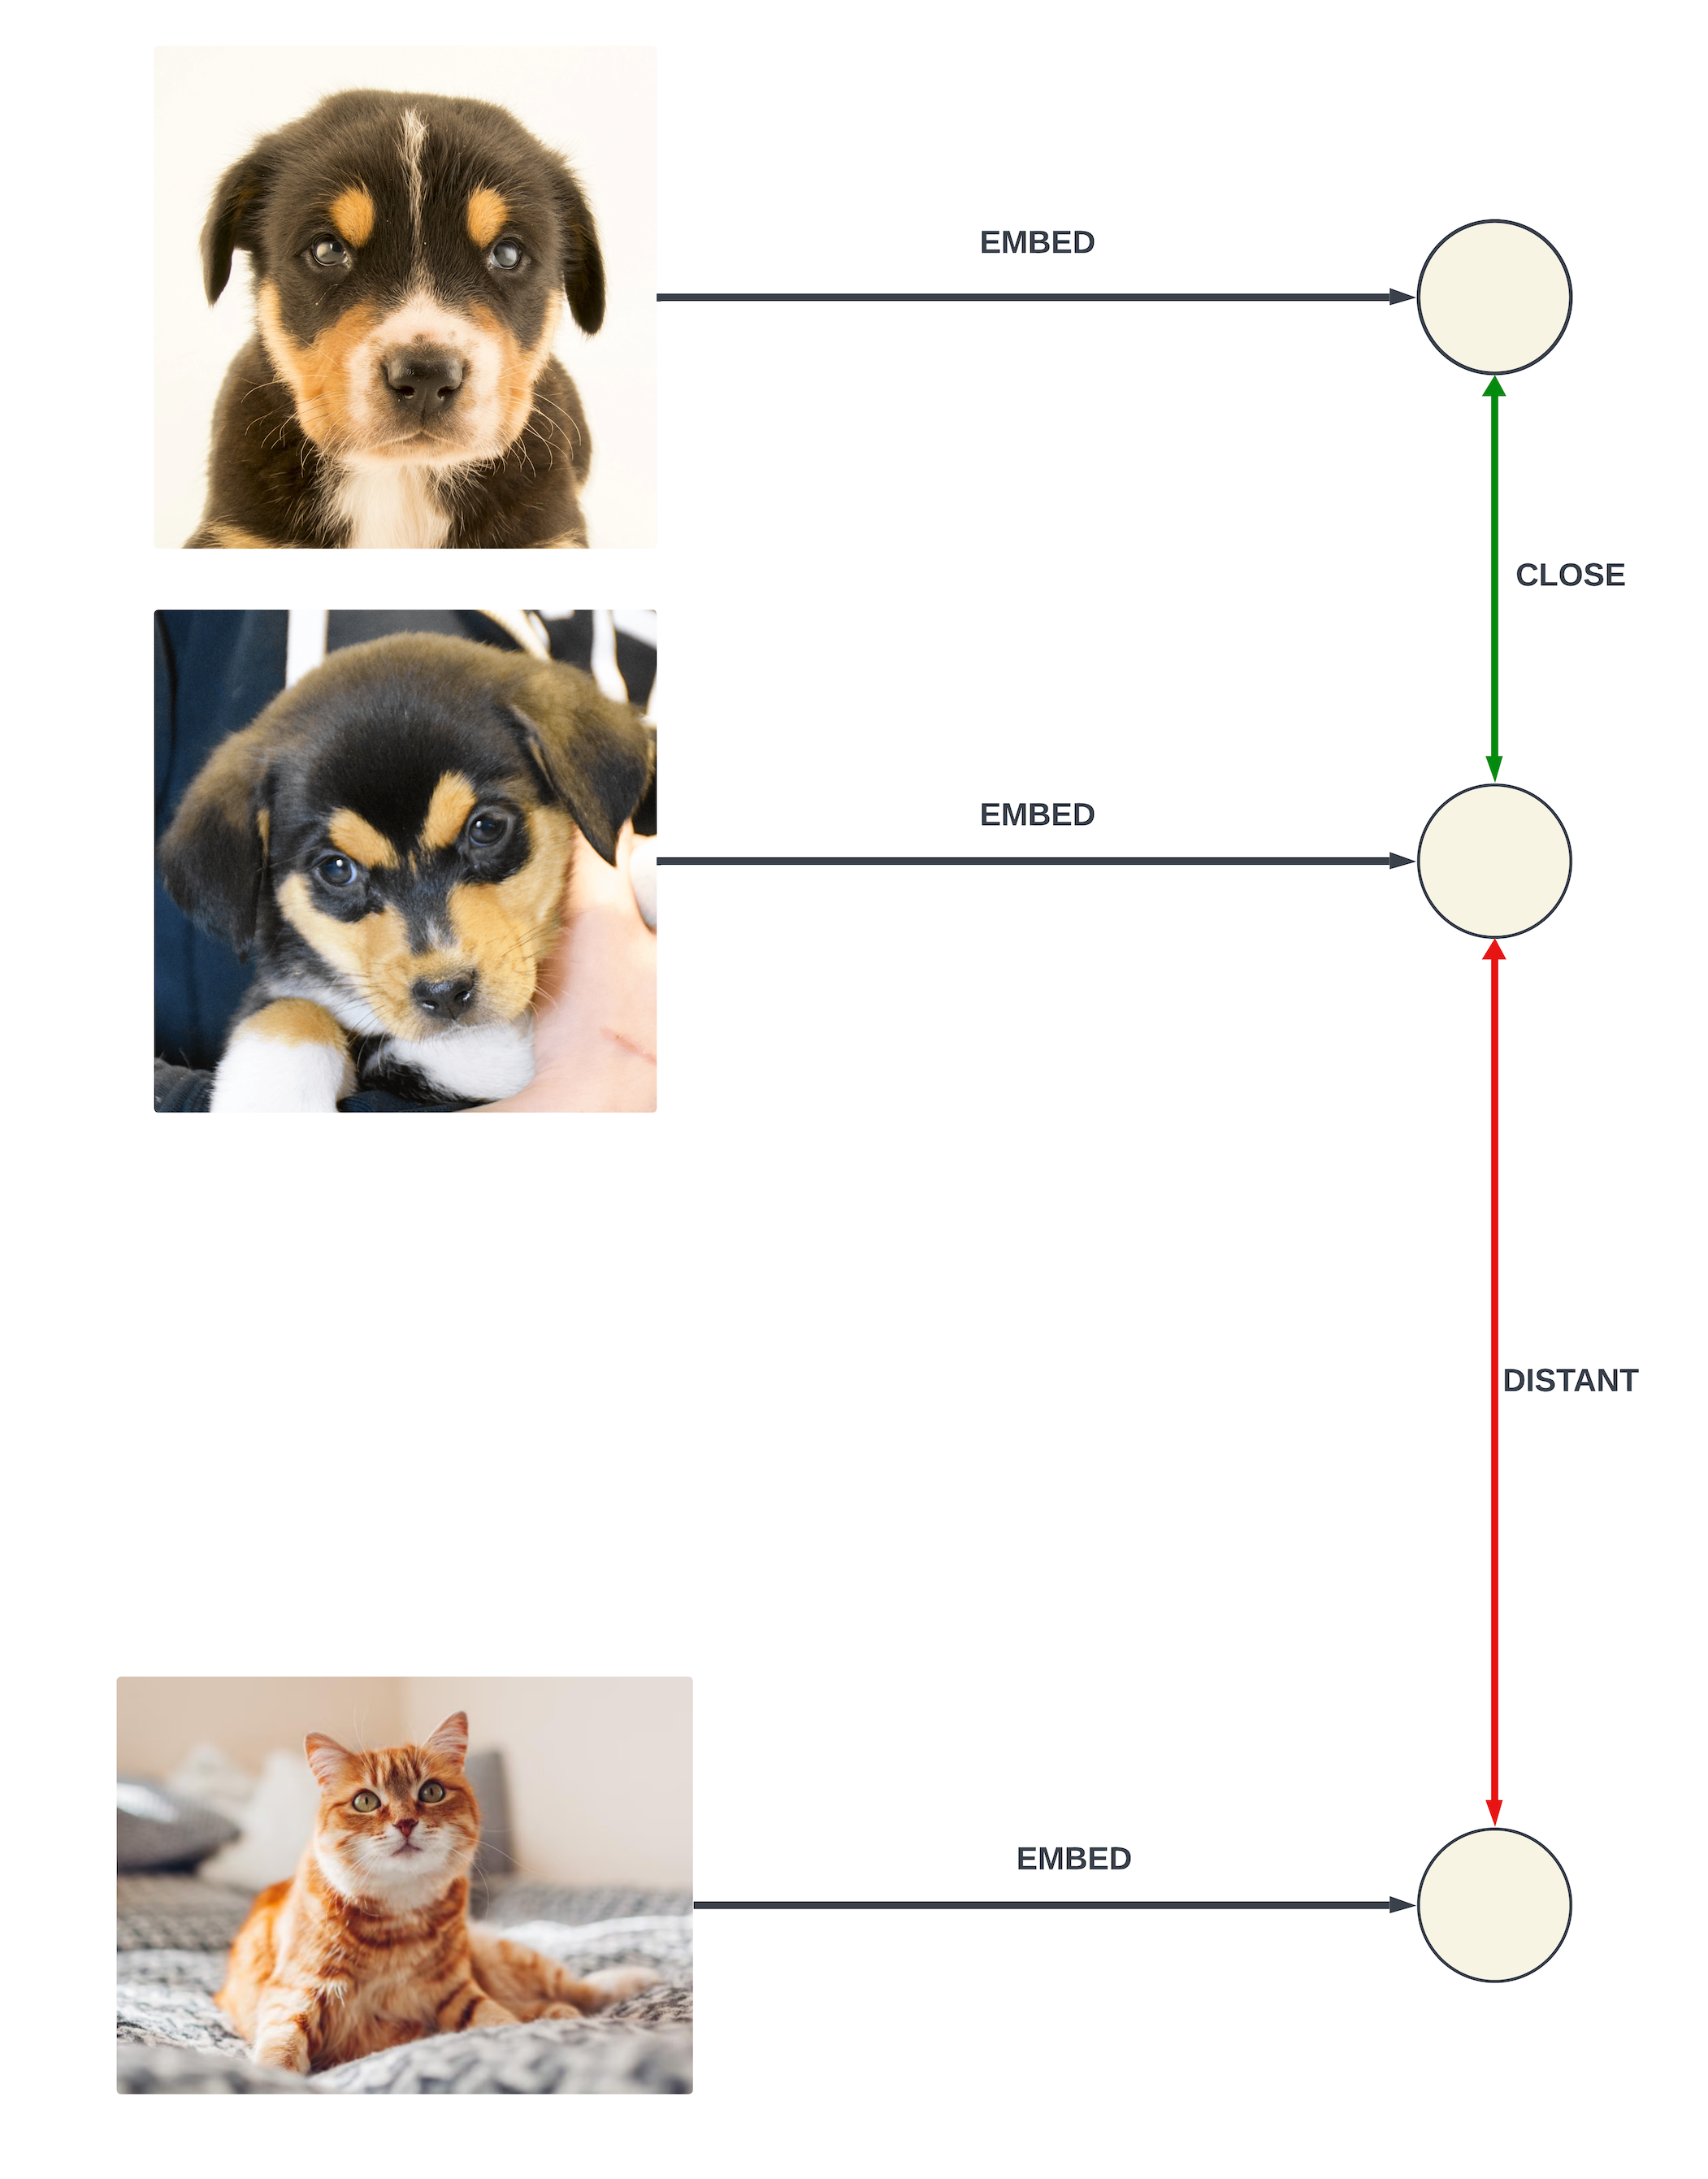
\includegraphics[height=3.4cm]{figure/contrastive-learning.png}
\end{figure}
\end{frame}

\begin{frame}{Contrastive Loss}
\begin{itemize}
  \item One of the first training objectives for contrastive learning. Input: a pair of samples, similar or dissimilar. Goal: map similar samples close in the embedding space, push dissimilar ones apart.
  \item For samples $x_i, x_j$ with classes $y_i, y_j$:
  $$L = \mathbb{1}[y_i = y_j]\,\|x_i - x_j\|^2 + \mathbb{1}[y_i \neq y_j]\,\max(0, \epsilon - \|x_i - x_j\|^2)$$
  \item If the samples are similar ($y_i = y_j$): minimize their squared Euclidean distance --- make them closer.
  \item If they are dissimilar ($y_i \neq y_j$): minimizing $\max(0, \epsilon - \|x_i - x_j\|^2)$ means maximizing their distance, up to a margin $\epsilon$.
\end{itemize}
\end{frame}

%%%%%%%%%%%%%%%%%%%%%%%%%%%%%%%%%%%%%%%%%%%%%%%%%%%%%%%%%%%%%%%%%%
\section{Contrastive Language-Image Pre-training (CLIP)}
% Source: HF CV course, unit4/multimodal-models/clip-and-relatives/clip
%%%%%%%%%%%%%%%%%%%%%%%%%%%%%%%%%%%%%%%%%%%%%%%%%%%%%%%%%%%%%%%%%%

\begin{frame}{CLIP}
\begin{itemize}
  \item CLIP \citebutton{Radford et al., 2021}{https://arxiv.org/abs/2103.00020} grasps visual concepts through \textbf{natural language supervision}: a text encoder and an image encoder are trained jointly on matching captions with their images.
  \item It adapts to a variety of visual classification benchmarks by simply receiving the \textit{names} of the visual categories to be recognized --- \enquote{zero-shot} capabilities akin to those of GPT-2 and GPT-3.
\end{itemize}
\end{frame}

\begin{frame}{Contrastive Pre-Training}
\begin{figure}
  \centering
  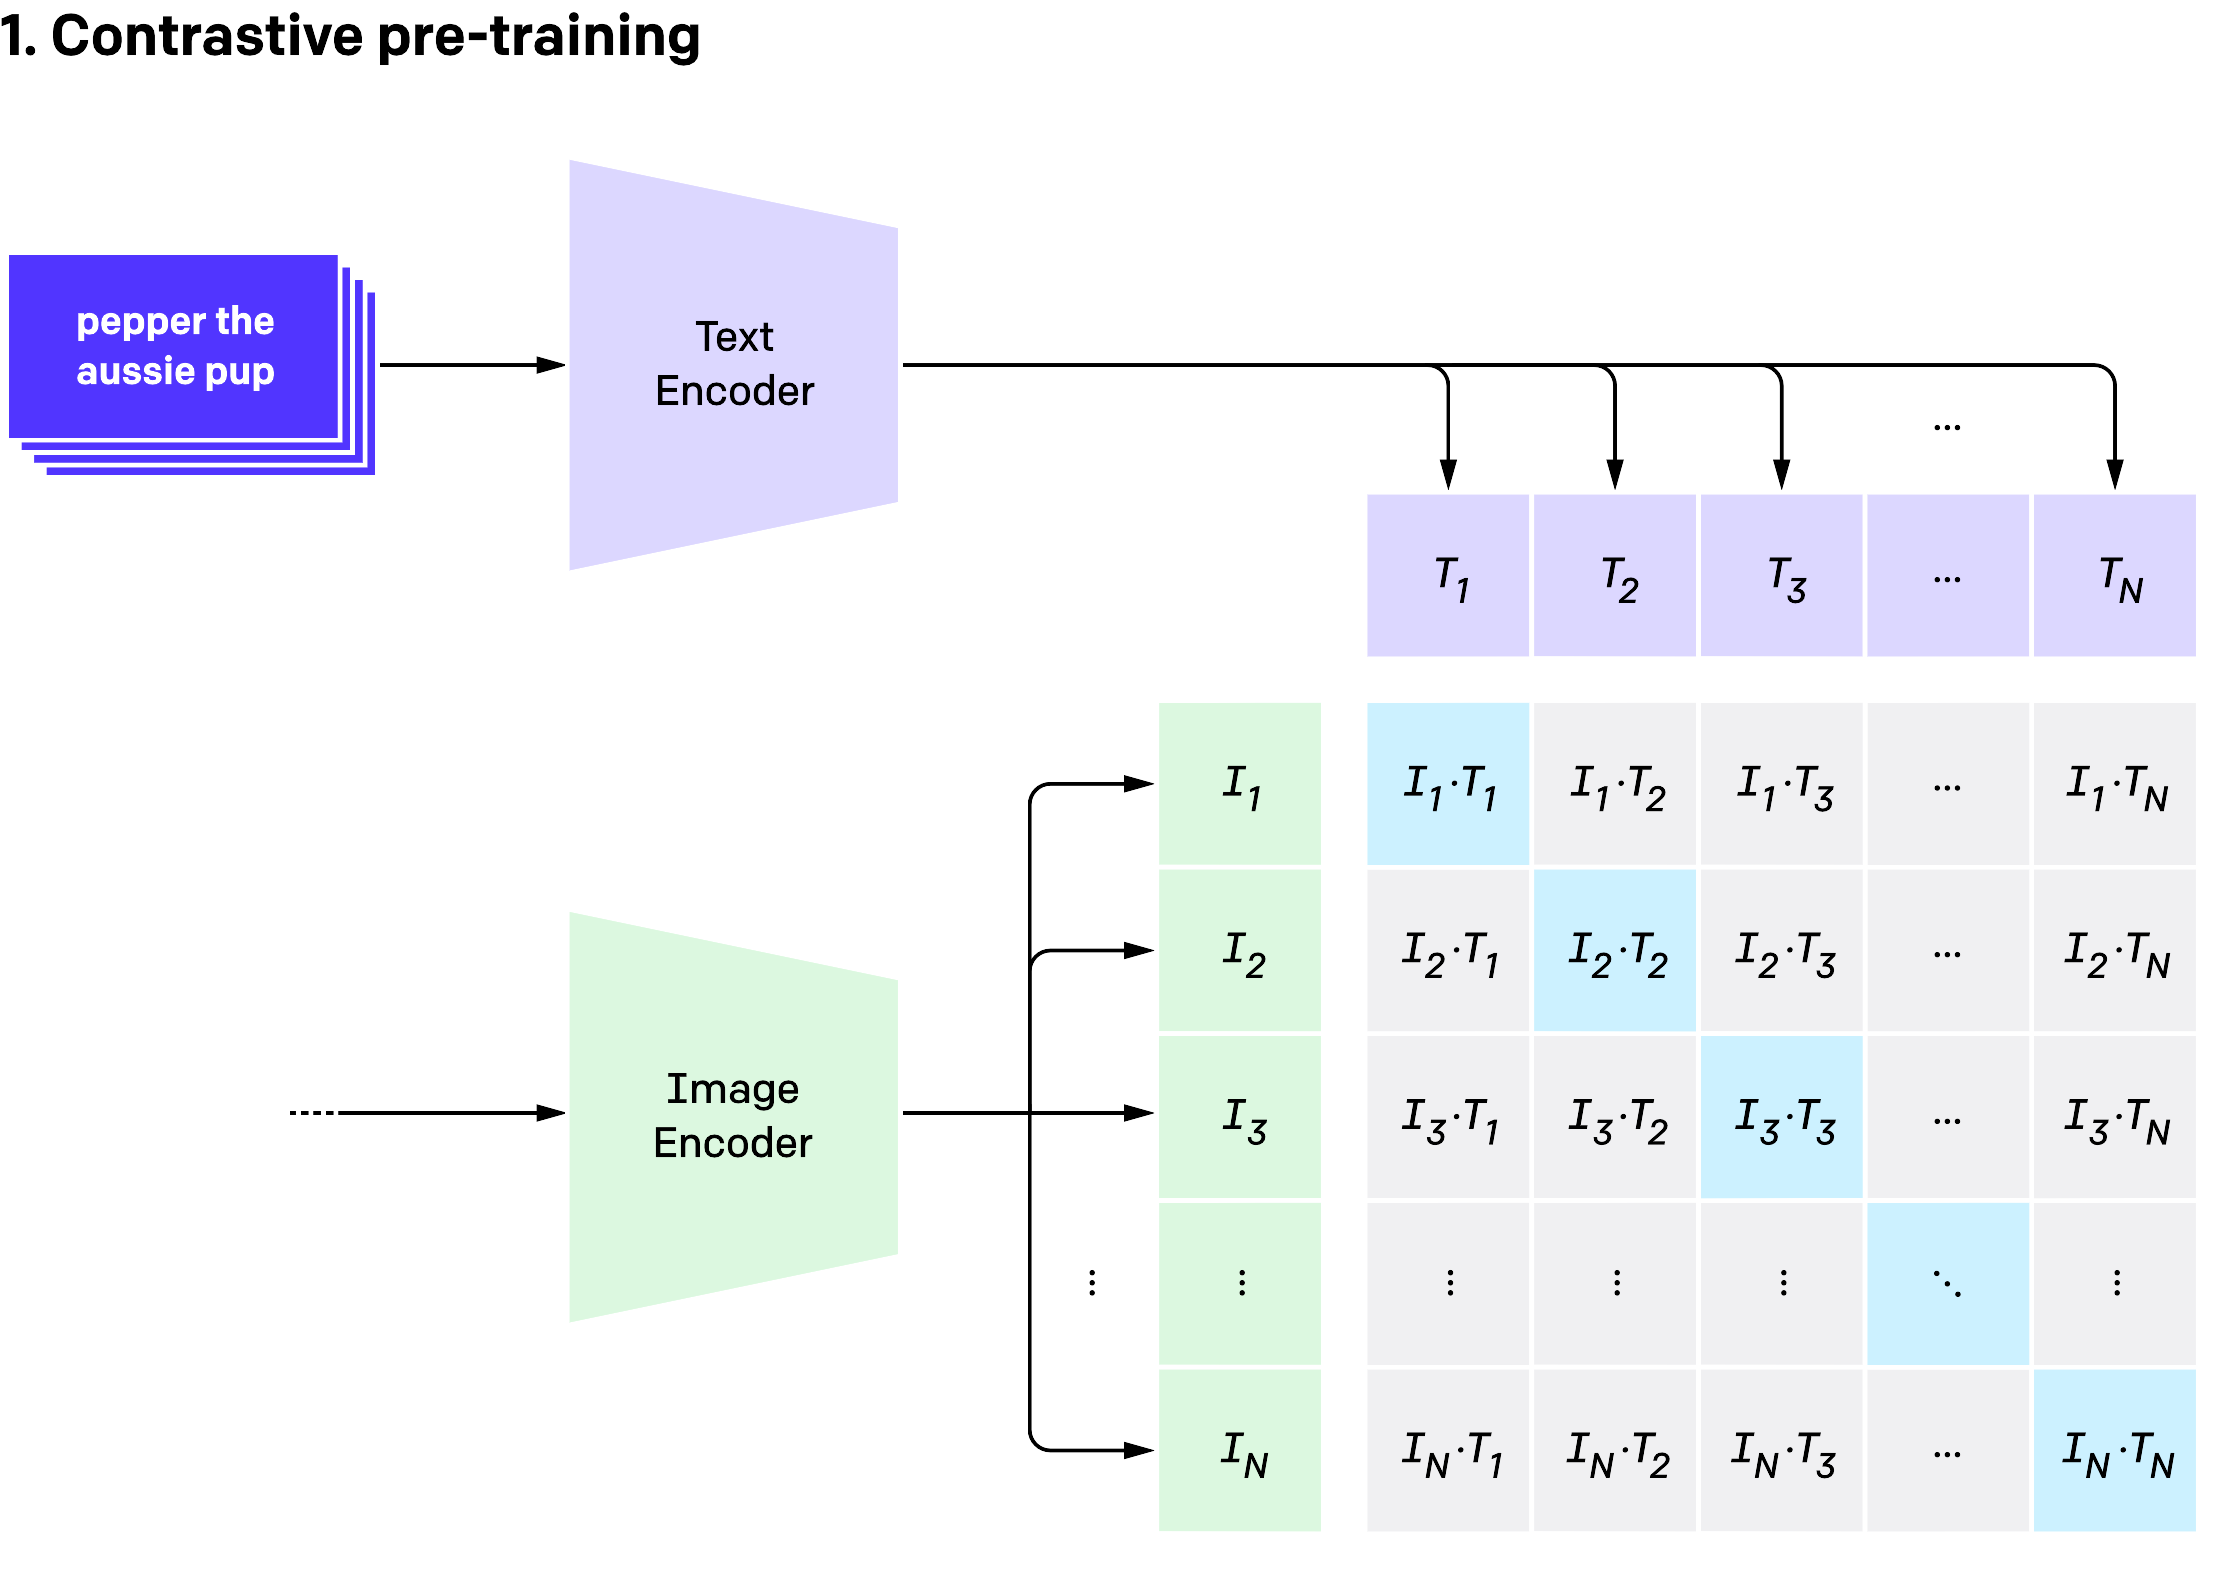
\includegraphics[height=2.80cm]{figure/clip-overview.png}\\
  \citebutton{Source: OpenAI}{https://openai.com/research/clip}
\end{figure}
\vspace{-0.3cm}
{\small
\begin{itemize}
  \item Given a batch of image-text pairs, compute the cosine similarity matrix between all possible (image, text) candidates.
  \item Maximize the similarity of correct pairs (blue diagonal), minimize it for incorrect pairs, via a \textbf{symmetric cross-entropy loss} over the similarity scores.
  \item In simple terms: each image should be most similar to its own caption, and each caption to its own image.
\end{itemize}
}
\end{frame}

\begin{frame}{CLIP: Encoders, Use Cases, Limitations}
\begin{itemize}
  \item \textbf{Independent encoders} for images and text: e.g.\ a Vision Transformer or a ResNet as image encoder. Switching an encoder requires retraining, as the embedding distribution changes.
  \item \textbf{Use cases}: zero-shot image classification, similarity search, conditioning diffusion models.
  \item \textbf{Limitations}:
  \begin{itemize}
    \item Unlikely to outperform a specialized, fine-tuned model; generalization is limited for data not encountered during training.
    \item Effectiveness and biases depend on the choice of categories: on the FairFace dataset, gender accuracy was over 96\%, racial accuracy around 93\%.
  \end{itemize}
\end{itemize}
\end{frame}

\begin{frame}[fragile]{CLIP: Zero-Shot Classification in Practice}
\scriptsize
\begin{verbatim}
from transformers import CLIPProcessor, CLIPModel

model = CLIPModel.from_pretrained("openai/clip-vit-base-patch32")
processor = CLIPProcessor.from_pretrained("openai/clip-vit-base-patch32")

inputs = processor(text=["a photo of a cat", "a photo of a dog"],
                   images=image, return_tensors="pt", padding=True)
outputs = model(**inputs)
probs = outputs.logits_per_image.softmax(dim=1)
\end{verbatim}
\normalsize
\begin{itemize}
  \item Zero-shot classification of a photo of cats between \texttt{dog} and \texttt{cat}: the class names become text prompts, and the image is matched against them.
  \item Result: \enquote{a photo of a cat} 99.49\%, \enquote{a photo of a dog} 0.51\%.
\end{itemize}
\end{frame}

%%%%%%%%%%%%%%%%%%%%%%%%%%%%%%%%%%%%%%%%%%%%%%%%%%%%%%%%%%%%%%%%%%
\section{Multimodal Text Generation (BLIP)}
% Source: HF CV course, unit4/multimodal-models/clip-and-relatives/blip
%%%%%%%%%%%%%%%%%%%%%%%%%%%%%%%%%%%%%%%%%%%%%%%%%%%%%%%%%%%%%%%%%%

\begin{frame}{BLIP: Bootstrapping Language-Image Pre-Training}
\begin{itemize}
  \item BLIP \citebutton{Li et al., 2022}{https://arxiv.org/abs/2201.12086} extends multimodal models to \textbf{text generation}.
  \item \textbf{CapFilt (caption and filtering)}: web-scraped image/alt-text pairs are noisy --- alt-texts often do not describe the image. One model filters out noisy pairs, another creates captions for images; both are first fine-tuned on a human-annotated dataset. Cleaning the data this way beat training on the raw web data.
  \item Takeaway: dataset \textbf{quality} matters, not just quantity.
  \item Successor: BLIP-2 \citebutton{Li et al., 2023}{https://arxiv.org/abs/2301.12597}, e.g.\ for visual question answering.
\end{itemize}
\end{frame}

\begin{frame}{BLIP: Architecture}
A vision encoder plus a \textbf{Multimodal mixture of Encoder-Decoder (MED)}:
\begin{itemize}
  \item \textbf{Vision Transformer}: a plain ViT with a {\tt [CLS]} token for the embedding.
  \item \textbf{Unimodal text encoder}: like BERT, with a {\tt [CLS]} token; trained with a contrastive loss like CLIP to align image and text representations.
  \item \textbf{Image-grounded text encoder}: {\tt [CLS]} replaced by an {\tt [Encode]} token; cross-attention layers combine image and text embeddings into a multimodal representation; a linear layer judges whether image and text match.
  \item \textbf{Image-grounded text decoder}: bidirectional self-attention replaced by \textbf{causal} self-attention; trained autoregressively with cross-entropy, for caption generation or visual question answering.
\end{itemize}
\end{frame}

%%%%%%%%%%%%%%%%%%%%%%%%%%%%%%%%%%%%%%%%%%%%%%%%%%%%%%%%%%%%%%%%%%
\section{Multipurpose Models}
% Source: LMU Multimodal Deep Learning booklet, ch. 4.3 (03-03-multi-purpose.Rmd),
% "Multipurpose Models" definition and "Overview of Multipurpose Models" incl. "Comparison". CC BY-NC-SA 4.0.
%%%%%%%%%%%%%%%%%%%%%%%%%%%%%%%%%%%%%%%%%%%%%%%%%%%%%%%%%%%%%%%%%%

\begin{frame}{Multipurpose Models}
\begin{itemize}
  \item \textbf{Multipurpose models} are multimodal-multitask models.
  \item They mimic human intelligence by marrying multiple perceptions and transferring knowledge about different tasks for better generalization.
  \item Main question: how is combining different modalities and tasks achieved?
  \item Four models: MultiModel (2017), UniT (2021), OFA (2022), Gato (2022).
\end{itemize}
\end{frame}

\begin{frame}{MultiModel}
\begin{itemize}
  \item A pre-Transformer-era model that combines architectural approaches from different fields. Four modules:
  \begin{itemize}
    \item \textbf{modality nets}: translate between real-world data and a unifying vector space (a tokenizer for language, convolutions for vision; also audio and categorical), and back for the output;
    \item \textbf{encoder}: receives the input from the modality nets and passes its output to the I/O mixer and the decoder;
    \item \textbf{I/O mixer} and \textbf{decoder}: combine their dual input using cross-attention; the decoder produces the output sequence autoregressively.
  \end{itemize}
  \item Trained on eight datasets (six language, plus COCO and ImageNet): below state-of-the-art and not significantly better than specialist models --- but much better on a low-resource task.
\end{itemize}
\end{frame}

\begin{frame}{Unified Transformer (UniT)}
\begin{itemize}
  \item Built on the Transformer with both encoder and decoder.
  \item \textbf{Modality-specific encoders}: BERT for text, a DETR encoder for vision (a CNN creates a lower-dimensional representation, reorganized as a sequence); more encoders may be added.
  \item A task-specific token is added to the encoder inputs; the encoder outputs are concatenated into a single sequence.
  \item The \textbf{decoder} follows DETR: it is fed task-specific query vectors instead of the previously produced sequence (not autoregressive); task-specific heads shape the output.
  \item The general model outperformed its single-task version on multimodal tasks but not on unimodal tasks; easily extendable by using available encoder models.
\end{itemize}
\end{frame}

\begin{frame}{OFA: Sequentialization Is All You Need}
\begin{itemize}
  \item All input is transformed into a \textbf{seq2seq problem} and embedded in a shared representation space --- no modality-specific modules.
  \item Images: as in ViT, flattened $16\times16$ patches, in the same dimension as the text token embeddings.
  \item Output: a sequence again --- images as a sequence of tokens, bounding boxes as a special sequence; another model turns the tokens into images or boxes.
  \item Autoregressive, cross-entropy loss; trained on cross-modal tasks (visual grounding, grounded captioning, image-text matching, captioning, VQA) and unimodal tasks.
  \item Outperformed state-of-the-art models on cross-modal tasks such as captioning and VQA; showed transfer to unseen tasks, but was not evaluated against a specialist baseline.
\end{itemize}
\end{frame}

\begin{frame}{Gato: A Generalist Decoder}
\begin{itemize}
  \item One model as a language model, an agent playing games, and an agent controlling robots: a \textbf{decoder-only} Transformer on a seq2seq problem.
  \item Every input is represented sequentially: images as $16\times16$ patches through a ResNet, text as tokens, game buttons and continuous robot movements tokenized in a vocabulary. A separator token ``$|$'' separates observations from the following action:
  \[ \left[\ \ldots \left[\, x_{\text{Text}},\, x_{\text{Images}},\, x_{\text{Discrete and Continuous Values}},\, |,\, y_{\text{Action}} \right]_i, \ldots \right] \]
\end{itemize}
\end{frame}

\begin{frame}{Gato: Training and Results}
\begin{itemize}
  \item The next action is predicted autoregressively; a mask in the cross-entropy loss restricts the loss to the action (for text, every token).
  \item Worse than specialist agents on reinforcement-learning tasks; on unseen tasks it needed fine-tuning, and the results were mixed: sometimes massive fine-tuning led only to small gains, but most of the time it outperformed the specialist agent.
\end{itemize}
\end{frame}

\begin{frame}{Multipurpose Models: Comparison}
\footnotesize
\resizebox{\textwidth}{!}{%
\begin{tabular}{@{}lllll@{}}
\toprule
Model & Approach & Modalities & Outperformed specialist? & Year \\
\midrule
OFA & Seq2Seq & Vision, Text & --- & 2022 \\
Gato & Seq2Seq & Vision, Text, Robotics, Discrete & In most cases & 2022 \\
UniT & $m$ encoders, task-specific head & Vision, Text & No & 2021 \\
MultiModel & Modality nets for Seq2Seq & Vision, Text, Audio, Categorical & Comparable & 2017 \\
\bottomrule
\end{tabular}%
}
\normalsize
\begin{itemize}
  \item A trend toward seq2seq models: the Transformer used entirely (OFA) or decoder-only (Gato), with a shared representation space and a particular ordering of input and output.
  \item UniT is more pragmatic: $m$ modalities encoded as a sequence, fused by the Transformer decoder.
  \item None besides OFA achieved state-of-the-art results; compared to specialists, the general models were comparable.
\end{itemize}
\end{frame}

%%%%%%%%%%%%%%%%%%%%%%%%%%%%%%%%%%%%%%%%%%%%%%%%%%%%%%%%%%%%%%%%%%
\section{Introduction to Video}
% Source: HF CV course, unit7/video-processing/introduction-to-video
%%%%%%%%%%%%%%%%%%%%%%%%%%%%%%%%%%%%%%%%%%%%%%%%%%%%%%%%%%%%%%%%%%

\begin{frame}{What Is a Video?}
\begin{itemize}
  \item An image is a two-dimensional representation of visual data; a \textbf{video} displays such frames sequentially --- played at a conventional speed, they give the illusion of motion (like a flipbook).
  \item Aspects of a video:
  \begin{itemize}
    \item \textbf{Resolution}: the number of pixels in each frame, e.g.\ HD ($1280\times720$), Full HD ($1920\times1080$), 4K ($3840\times2160$). More detail, but more storage and processing power.
    \item \textbf{Frame rate}: frames displayed per second, commonly 24, 30, 60 fps. Higher frame rates give smoother motion.
    \item \textbf{Bitrate}: the quantity of data needed to describe audio and video; higher bitrate, better quality, more storage and bandwidth.
    \item \textbf{Codecs} (compressor-decompressor): lossless or lossy compression of digital media.
  \end{itemize}
\end{itemize}
\end{frame}

\begin{frame}{Video Processing}
\begin{itemize}
  \item Video processing automatically analyzes video data to understand and interpret both \textbf{temporal and spatial} features: video is a sequence of time-varying images, digitized both spatially and temporally.
  \item Traditionally, deep learning research focused on images, speech, and text; video offers a valuable opportunity due to its size and complexity.
  \item Applications:
  \begin{itemize}
    \item \textbf{surveillance}: public safety, crime prevention, traffic monitoring;
    \item \textbf{autonomous driving}: navigation, obstacle detection, recognizing road signs;
    \item \textbf{healthcare}: diagnostics, feedback during surgery, patient monitoring.
  \end{itemize}
\end{itemize}
\end{frame}

\begin{frame}{Challenges in Video Processing}
\begin{itemize}
  \item \textbf{Computational demands}: real-time video analysis requires substantial processing power.
  \item \textbf{Storage requirements}: high-resolution videos generate large volumes of data; efficient compression and data management are necessary.
  \item \textbf{Privacy and ethical concerns}: especially in surveillance and healthcare, video processing handles sensitive information.
\end{itemize}
\end{frame}

%%%%%%%%%%%%%%%%%%%%%%%%%%%%%%%%%%%%%%%%%%%%%%%%%%%%%%%%%%%%%%%%%%
\section{Transformers in Video Processing}
% Source: HF CV course, unit7/video-processing/transformers-based-models
%%%%%%%%%%%%%%%%%%%%%%%%%%%%%%%%%%%%%%%%%%%%%%%%%%%%%%%%%%%%%%%%%%

\begin{frame}{ViT: Performance and Limitation}
\begin{figure}
  \centering
  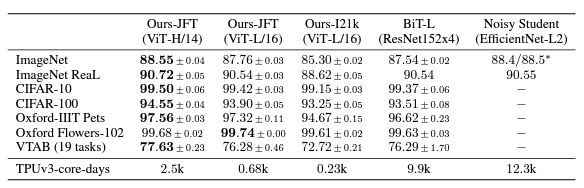
\includegraphics[width=0.75\textwidth]{figure/vit-performance.jpg}\\
  \citebutton{Source: Dosovitskiy et al., 2020}{https://arxiv.org/abs/2010.11929}
\end{figure}
\begin{itemize}
  \item ViT outperformed other state-of-the-art models, but training it required 2{,}500 TPU-v3 days. At roughly \$2 per TPU-v3 core-hour, one training run costs about $2 \times 24 \times 2500 = $ \$120{,}000.
\end{itemize}
\end{frame}

\begin{frame}{Video Vision Transformer (ViViT)}
\begin{itemize}
  \item ViViT \citebutton{Arnab et al., 2021}{https://arxiv.org/abs/2103.15691} extends ViT to video classification. Key issues: train more quickly and efficiently, and handle \textbf{temporal} as well as spatial information.
  \item Extracts spatio-temporal tokens from the video and encodes them with Transformer layers; efficient variants factorise the spatial and temporal dimensions; pre-trained image models make training on comparatively small datasets possible.
\end{itemize}
\begin{figure}
  \centering
  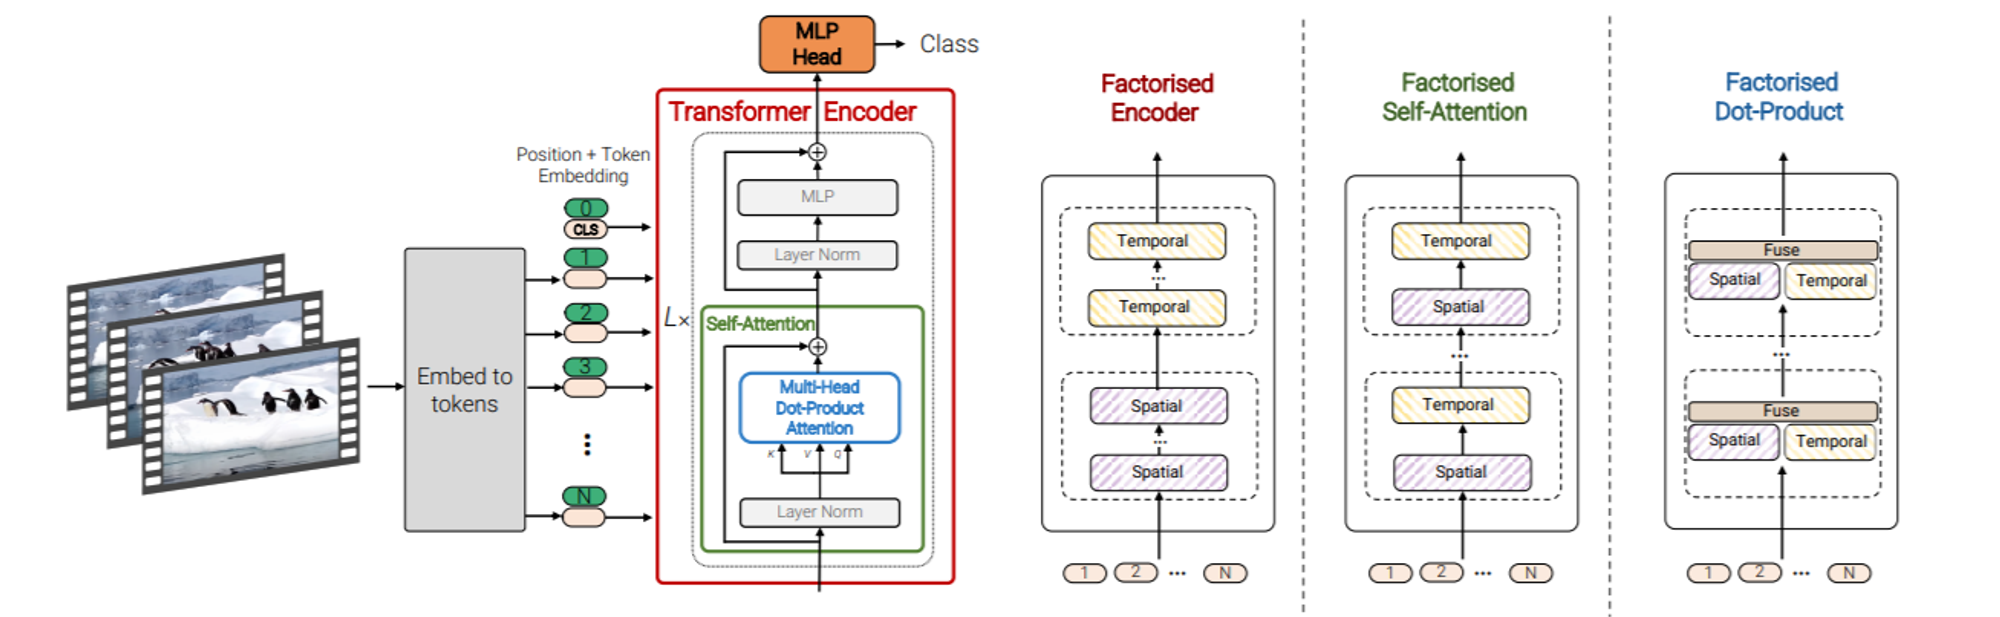
\includegraphics[width=0.72\textwidth]{figure/vivit-architecture.png}\\
  \citebutton{Source: Arnab et al., 2021}{https://arxiv.org/abs/2103.15691}
\end{figure}
\end{frame}

\begin{frame}{Embedding Video Clips}
\begin{itemize}
  \item Embeddings: dense vectors capturing meaningful features. For video, they must preserve \textbf{spatial} (what is in each frame) and \textbf{temporal} (how things change) information, while reducing dimensionality so processing stays feasible.
\end{itemize}
\begin{columns}
\begin{column}{0.48\textwidth}
\centering
\textbf{Uniform frame sampling}\\
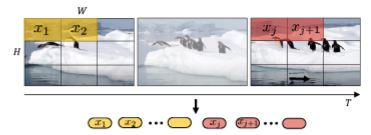
\includegraphics[width=0.8\textwidth]{figure/vivit-uniform-sampling.jpg}\\
{\footnotesize Sample frames uniformly over time, e.g.\ one in every 2 frames.}
\end{column}
\begin{column}{0.48\textwidth}
\centering
\textbf{Tubelet embedding}\\
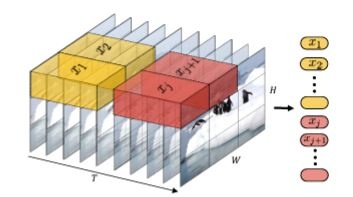
\includegraphics[width=0.8\textwidth]{figure/vivit-tubelet.jpg}\\
{\footnotesize Extract spatio-temporal \enquote{tubes} and project them linearly: fuses space and time already during tokenization.}
\end{column}
\end{columns}
\vspace{0.1cm}
{\footnotesize Figures: \citebutton{Arnab et al., 2021}{https://arxiv.org/abs/2103.15691}}
\end{frame}

\begin{frame}{ViViT Model 1: Spatio-Temporal Attention}
\begin{itemize}
  \item The natural extension of ViT: each of the $n_t$ frames is split into $n_w \times n_h$ patches, giving $n_t \times n_w \times n_h$ \textbf{spatio-temporal tokens}.
  \item All tokens go through the Transformer encoder together, so each token is contextualized with all others across space and time --- patterns in position, color and movement.
  \item Complexity: $\mathcal{O}(n_h^2\, n_w^2\, n_t^2)$.
  \item Attention over all spatio-temporal tokens is expensive; uniform frame sampling and tubelet embedding help reduce the cost.
\end{itemize}
\end{frame}

\begin{frame}{ViViT Model 2: Factorised Encoder}
\begin{figure}
  \centering
  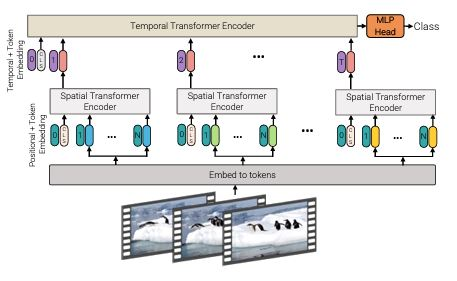
\includegraphics[height=2.9cm]{figure/vivit-model2.jpg}\\
  \citebutton{Source: Arnab et al., 2021}{https://arxiv.org/abs/2103.15691}
\end{figure}
\vspace{-0.3cm}
{\small
\begin{itemize}
  \item Model 1 contextualizes all patches simultaneously --- inefficient. Model 2 separates spatial and temporal encoders, sequentially:
  \begin{itemize}
    \item a \textbf{spatial} Transformer encoder (= ViT) contextualizes within each frame and encodes it into a single embedding;
    \item a \textbf{temporal} Transformer encoder then processes the frame embeddings.
  \end{itemize}
  \item Complexity: $\mathcal{O}(n_h^2\, n_w^2 + n_t^2)$.
\end{itemize}
}
\end{frame}

\begin{frame}{ViViT Models 3 and 4}
\begin{columns}
\begin{column}{0.48\textwidth}
\centering
\textbf{Model 3: Factorised Self-Attention}\\
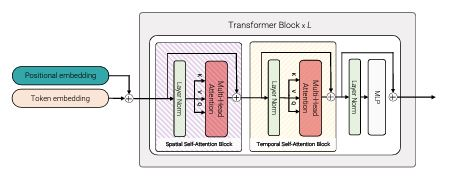
\includegraphics[width=0.85\textwidth]{figure/vivit-model3.jpg}\\
{\footnotesize First self-attention \textbf{spatially} (among tokens of the same time index), then \textbf{temporally} (among tokens of the same spatial index). No {\tt [CLS]} token, because of ambiguities.}
\end{column}
\begin{column}{0.48\textwidth}
\centering
\textbf{Model 4: Factorised Dot-Product Attention}\\
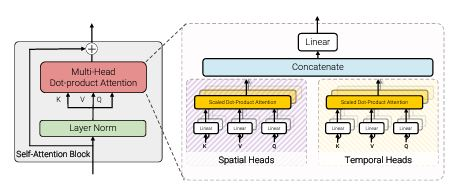
\includegraphics[width=0.85\textwidth]{figure/vivit-model4.jpg}\\
{\footnotesize Half of the attention heads use keys and values from the same spatial indices, the other half from the same temporal indices.}
\end{column}
\end{columns}
\vspace{0.1cm}
{\footnotesize Complexity of both: same as Model 2. Figures: \citebutton{Arnab et al., 2021}{https://arxiv.org/abs/2103.15691}}
\end{frame}

\begin{frame}{ViViT: Experiments and Discussion}
\begin{figure}
  \centering
  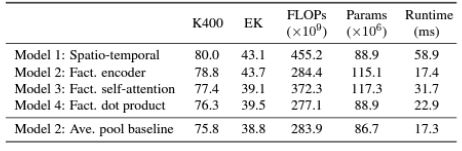
\includegraphics[width=0.55\textwidth]{figure/vivit-performance.jpg}\\
  \citebutton{Source: Arnab et al., 2021}{https://arxiv.org/abs/2103.15691}
\end{figure}
\begin{itemize}
  \item Model 1 achieves the best accuracy but needs the longest training; Model 2 gives relatively high accuracy with shorter training than Models 3 and 4 --- the most efficient overall.
  \item Like ViT, ViViT needs extremely large datasets, which rarely exist for video. Approach: first pre-train on a large image dataset with ViT to initialize the model.
\end{itemize}
\end{frame}

\begin{frame}{TimeSformer}
Concurrent work with ViViT \citebutton{Bertasius et al., 2021}{https://arxiv.org/abs/2102.05095}; five space-time self-attention schemes (blue: query patch):
\begin{figure}
  \centering
  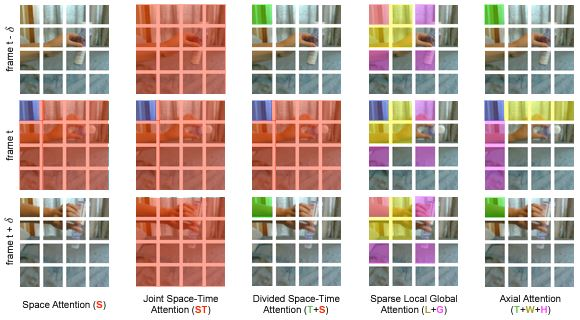
\includegraphics[height=1.88cm]{figure/timesformer.jpg}
\end{figure}
\vspace{-0.3cm}
{\small
\begin{itemize}
  \item \textbf{Space}: as in ViT, within one frame. \textbf{Joint space-time}: across frames, as ViViT Model 1.
  \item \textbf{Divided space-time}: first temporally (same position, other frames), then spatially --- similar to ViViT Model 3.
  \item \textbf{Sparse local global}: selectively combines local and global information. \textbf{Axial}: spatial and temporal dimensions separately along their axes.
  \item \textbf{Divided space-time attention} gives the best balance of parameter efficiency and accuracy (K400, SSv2).
\end{itemize}
}
\end{frame}

\begin{frame}{Conclusion: Video Transformers}
\begin{itemize}
  \item ViViT extended ViT to video with several models (factorised encoder, factorised self-attention, factorised dot-product attention), all aimed at managing the space-time dimensions efficiently.
  \item TimeSformer likewise evolved from ViT, using diverse attention mechanisms over space and time.
  \item Key takeaway: the focus is on reducing the significant computational cost of applying Transformers to video, enabling learning with fewer computational resources.
\end{itemize}
\end{frame}

%%%%%%%%%%%%%%%%%%%%%%%%%%%%%%%%%%%%%%%%%%%%%%%%%%%%%%%%%%%%%%%%%%
\section{License \& Attribution}
%%%%%%%%%%%%%%%%%%%%%%%%%%%%%%%%%%%%%%%%%%%%%%%%%%%%%%%%%%%%%%%%%%

\begin{frame}[shrink=30]{License \& Attribution}
% fit16:9: shrink (the itemize template ignores \small here)
\begin{itemize}
\item \textbf{Main source.} All sections except those listed below follow the \textbf{Hugging Face Community Computer Vision Course} (\url{https://huggingface.co/learn/computer-vision-course}, repository \url{https://github.com/johko/computer-vision-course}, \copyright\ 2023 Johannes Kolbe and contributors) --- licensed \textbf{MIT}. Units 1 (\textit{Introduction}), 3 (\textit{Vision Transformers}), 4 (\textit{Multimodal Models}) and 7 (\textit{Video}). The course is prose, not slides: frames condense its text into bullet points without adding content.
\item \textbf{Supplement.} \enquote{Transformers in Computer Vision}, \enquote{Multimodal Architectures} and \enquote{Multipurpose Models} condense text from the LMU booklet \textbf{\textit{Multimodal Deep Learning}} (SLDS, LMU Munich, \url{https://slds-lmu.github.io/seminar_multimodal_dl/}, chapters 2.2, 3 and 4.3) --- licensed \textbf{CC BY-NC-SA 4.0} (\url{https://creativecommons.org/licenses/by-nc-sa/4.0/}): non-commercial use, with attribution; these three sections are adapted from it and are therefore shared under the same license. The ViT figure in that section is from the booklet, which takes it from the paper.
\item \textbf{Figures} are those the course uses, with the attribution the course gives: most are taken from the original papers (linked on each frame); the CLIP pre-training figure is from OpenAI; the MaskFormer figure comes via the Hugging Face documentation.
\end{itemize}
\end{frame}

\endlecture
\end{document}
